\documentclass[a4paper,12pt]{article}
\usepackage[utf8]{inputenc}
\usepackage[german]{babel}
\usepackage{amsmath}
\usepackage{amssymb}
\usepackage{amsthm}
\usepackage{geometry}
\usepackage{graphicx}
\usepackage[hidelinks]{hyperref}
\usepackage{listings}
\usepackage{xcolor}
\usepackage{enumitem}
\usepackage{microtype}
\usepackage{longtable}
\usepackage{booktabs}

\geometry{margin=2.5cm}

\sloppy
\emergencystretch=3em

\theoremstyle{definition}
\newtheorem{definition}{Definition}
\newtheorem{beispiel}{Beispiel}
\newtheorem{satz}{Satz}
\newtheorem{lemma}{Lemma}
\newtheorem{korollar}{Korollar}
\newtheorem{bemerkung}{Bemerkung}

\setlist[itemize,1]{label=--}

% ---------- Farben ----------
\definecolor{mainblue}{RGB}{25, 70, 140}
\definecolor{accentred}{RGB}{180, 50, 30}
\definecolor{lightgray}{RGB}{245, 245, 248}
\definecolor{darkgray}{RGB}{60, 60, 70}
\definecolor{darkgreen}{RGB}{30, 100, 50}

\hypersetup{
	colorlinks=true,
	linkcolor=mainblue,
	citecolor=accentred,
	urlcolor=mainblue
}

%  Code-Highlighting
\lstset{
	basicstyle=\ttfamily\small,
	keywordstyle=\color{blue},
	commentstyle=\color{gray},
	stringstyle=\color{red},
	numbers=left,
	numberstyle=\tiny,
	breaklines=true,
	breakatwhitespace=false,
	frame=single,
	columns=fullflexible,
	literate=%
	{Ö}{{\"O}}1
	{Ä}{{\"A}}1
	{Ü}{{\"U}}1
	{ß}{{\ss}}1
	{ü}{{\"u}}1
	{ä}{{\"a}}1
	{ö}{{\"o}}1
	{Σ}{{$\Sigma$}}1
	{σ}{{$\sigma$}}1
	{→}{{$\rightarrow$}}1
	{⊆}{{$\subseteq$}}1
	{⊇}{{$\supseteq$}}1
	{≥}{{$\geq$}}1
}

\title{\textbf{Inbetriebnahme eines}\\[0.2em]\textbf{Hardware Security Module}\\[0.3em]
\large Ein kryptographischer HSM-Funktionskern für den Infineon AURIX TC3x,\\
abgeleitet aus der Signatur-Chiffre und dem Fenster-Chiffre-Protokoll}
\author{Stephan Epp}
\date{30. Juni 2026}

\begin{document}

\maketitle

\begin{abstract}
\noindent
Diese Arbeit überträgt die in \cite{Epp26b} (Signatur-Chiffre) und \cite{Epp26c} (Fenster-Chiffre, wchiffre) formal entwickelten kryptographischen Verfahren in einen konkreten Hardware-Funktionsentwurf für das Hardware Security Module (HSM) der Infineon-AURIX-TC3x-Mikrocontrollerfamilie. Ausgehend von der injektiven Signaturfunktion $\sigma$ und der affinen Modulartransformation $(a,b,p)$ wird ein vollständiger Satz von zehn HSM-Hardwarefunktionen spezifiziert: Schlüsselerzeugung, Signatur, Verifikation, symmetrische Modularverschlüsselung, Secure-Boot-Verifikation, Firmware-Integritätsprüfung über Subgraph-Signaturen sowie ein True Random Number Generator als gemeinsame Entropiequelle. Für jede Funktion werden formale Korrektheitsbeweise, eine Komplexitäts- und Sicherheitsanalyse sowie eine Abschätzung von Taktzyklen, Energiebedarf und Speicherbedarf auf der TriCore-Lockstep-Architektur vorgenommen. Die Ergebnisse werden durch acht matplotlib-Diagramme veranschaulicht. Die Arbeit schließt mit einer sehr ausführlichen Betrachtung des Ausblicks, insbesondere zur Integration gitterbasierter Post-Quanten-Verfahren und zur Seitenkanalhärtung.
\end{abstract}

\tableofcontents
\newpage

\section{Einführung}

\subsection{Motivation}

Hardware Security Module (HSM) sind dedizierte, vom Applikationskern getrennte Recheneinheiten innerhalb moderner Mikrocontroller, die kryptographische Operationen, Schlüsselverwaltung und Boot-Integritätsprüfung isoliert und manipulationssicher ausführen. Die AURIX-TC3x-Familie von Infineon integriert ein solches HSM als eigenständigen, abgesicherten TriCore-Kern mit eigenem Flash-, RAM- und Peripheriebereich, der über die HSI-Schnittstelle (\emph{Hardware Security Interface}) mit den Applikationskernen kommuniziert.

In der Praxis werden HSM-Bausteine bislang überwiegend mit etablierten symmetrischen und asymmetrischen Standardverfahren (AES, RSA, ECC) ausgelegt. Die vorliegende Arbeit verfolgt einen anderen Ansatz: Sie legt die Funktionen des HSM \emph{maßgeblich} anhand der in den Arbeiten \cite{Epp26b,Epp26c} entwickelten eigenen kryptographischen Primitive aus -- der Signatur-Chiffre und des Fenster-Chiffre-Protokolls -- und erweitert diese um eine hardwarenahe Spezifikation, formale Korrektheitsbeweise auf Registerebene sowie eine quantitative Hardware-Kostenanalyse.

\subsection{Beitrag dieser Arbeit}

\begin{itemize}
	\item Eine vollständige funktionale Architektur des HSM-Kryptographiekerns mit zehn klar abgegrenzten Hardwarefunktionen (Abschnitt~\ref{sec:funktionen}).
	\item Formale Ãœbertragung der Signaturfunktion $\sigma$, der affinen Transformation und des Fenster-Protokolls in ein Register-Transfer-Modell (Abschnitt~\ref{sec:hwmodell}).
	\item Korrektheits- und Sicherheitsbeweise für jede HSM-Funktion, aufbauend auf den in \cite{Epp26b,Epp26c,Epp26a} etablierten Sätzen (Abschnitt~\ref{sec:korrektheit}).
	\item Eine Komplexitäts-, Energie- und Speicheranalyse auf Basis der TriCore-Lockstep-Architektur (Abschnitt~\ref{sec:analyse}).
	\item Acht experimentelle Visualisierungen (Abschnitt~\ref{sec:experimente}) sowie ein sehr ausführlicher Ausblick (Abschnitt~\ref{sec:ausblick}) zur Weiterentwicklung, insbesondere Richtung Post-Quanten-Kryptographie und Seitenkanalresistenz.
\end{itemize}

\subsection{Struktur der Arbeit}

Abschnitt~\ref{sec:grundlagen} fasst die mathematischen Grundlagen aus der Signatur-Chiffre und dem Fenster-Chiffre-Protokoll zusammen (injektive Signaturfunktion, Modulararithmetik über $\mathbb{Z}_p$, Fenster-Protokoll, gitterbasierte Erweiterung). Abschnitt~\ref{sec:hwmodell} führt das Hardwaremodell des TC3x-HSM ein (Systemarchitektur, Funktionseinheiten, Registermodell, Zustandsmaschine). Abschnitt~\ref{sec:funktionen} spezifiziert alle zehn HSM-Funktionen im Detail (\texttt{TRNG\_Read}, \texttt{SignatureCipher\_KeyGen/Sign/Verify}, \texttt{ModularCipher\_Encrypt/Decrypt}, \texttt{SubgraphSig\_Derive}, \texttt{SecureBoot\_Verify}, \texttt{KeyStore\_Provision/Lock}). Abschnitt~\ref{sec:korrektheit} liefert die formalen Korrektheits- und Sicherheitsbeweise für alle Funktionen. Abschnitt~\ref{sec:analyse} enthält die Komplexitäts-, Energie- und Speicheranalyse auf der TriCore-Lockstep-Architektur. Abschnitt~\ref{sec:experimente} veranschaulicht alle Ergebnisse mit neun matplotlib-Diagrammen. Abschnitt~\ref{sec:radar} wertet formal die Secure-Boot-Verifikationszeit für ein Radar-ECU mit $4$\,MB Programm-Flash aus ($\approx 7\,340$\,ms sequenziell). Abschnitt~\ref{sec:parallel} spezifiziert und beweist die $k$-fache parallele Sig-Engine-Architektur, die diese Verifikationszeit auf $\approx 459$\,ms ($k=16$) reduziert. Abschnitt~\ref{sec:ausblick} schließt mit einem sehr ausführlichen Ausblick über neun Weiterentwicklungsrichtungen. Die Zusammenfassung fasst alle Ergebnisse ab, gefolgt vom Literaturverzeichnis.


\section{Mathematische Grundlagen}
\label{sec:grundlagen}

Dieser Abschnitt rekapituliert kurz und formal die Bausteine aus \cite{Epp26b,Epp26c,Epp26a}, die im Hardwareentwurf direkt als Funktionseinheiten realisiert werden. Auf ausführliche Beweise wird hier verzichtet und stattdessen auf die Originalarbeiten verwiesen; die für den HSM-Entwurf \emph{neuen} Sätze werden in Abschnitt~\ref{sec:korrektheit} vollständig beweisen.

\subsection{Die injektive Signaturfunktion}

\begin{definition}[Signaturfunktion, nach \cite{Epp26a,Epp26b}]
	\label{def:sigma}
	Sei $A \in \{0,1\}^{n \times n}$ eine binäre Matrix und $j \in \{0,\ldots,n-1\}$ ein Spaltenindex. Die \textbf{Signaturfunktion} ist
	\[
	\sigma(A, j) := \sum_{i=0}^{n-1} A_{ij} \cdot 2^i + j \cdot 2^n.
	\]
\end{definition}

\begin{lemma}[Injektivität, nach \cite{Epp26a,Epp26b}]
	\label{lem:inj}
	Aus $\sigma(A,j) = \sigma(A',j')$ folgt $j=j'$ und $A_{\cdot j} = A'_{\cdot j'}$.
\end{lemma}

Im Hardwarekontext ist Lemma~\ref{lem:inj} deshalb von Bedeutung, weil die Signaturfunktion in der Funktion \texttt{HSM\_SubgraphSig\_Derive} (Abschnitt~\ref{sec:funk-subgraphsig}) zur eindeutigen, kollisionsfreien Ableitung eines Integritätswertes aus dem Firmware-Abbild verwendet wird: Zwei verschiedene Firmware-Spalten können niemals dieselbe Signatur erzeugen.

\subsection{Modulare Arithmetik über $\mathbb{Z}_p$}

\begin{definition}[Schlüssel der Signatur-Chiffre, nach \cite{Epp26b}]
	\label{def:schluessel}
	Ein Signatur-Chiffre-Schlüssel ist ein Tripel $(a,b,p)$ mit $p$ prim, $p > 2^{2n}$, $a \in \mathbb{Z}_p^*$, $b \in \mathbb{Z}_p$. Verschlüsselung und Entschlüsselung erfolgen über die Bijektion
	\[
	f(x) = (ax+b) \bmod p, \qquad f^{-1}(y) = a^{-1}(y-b) \bmod p.
	\]
\end{definition}

\begin{satz}[$\mathbb{Z}_p$ ist ein Körper, nach \cite{Epp26b}]
	\label{satz:koerper}
	Ist $p$ prim, so besitzt jedes $a \in \mathbb{Z}_p \setminus \{0\}$ ein eindeutiges multiplikatives Inverses, berechenbar in $O(\log p)$ Schritten mit dem erweiterten euklidischen Algorithmus.
\end{satz}

Satz~\ref{satz:koerper} ist die mathematische Grundlage der Hardwarefunktionseinheit \texttt{Modular-ALU} (Abschnitt~\ref{sec:hwmodell}): Sie implementiert den erweiterten euklidischen Algorithmus als feste Mikrocode-Sequenz zur Inversenberechnung bei der Schlüsselerzeugung.

\subsection{Das Fenster-Chiffre-Protokoll}

Das in \cite{Epp26c} eingeführte Fenster-Chiffre-Protokoll (wchiffre) kombiniert die Einheitengruppe $\mathbb{Z}_{32}^*$, eine RSA-artige asymmetrische Komponente und ein Dummy-Paket-Schema zur Verschleierung des tatsächlichen Nachrichtenverkehrs.

\begin{definition}[Einheitengruppe modulo 32, nach \cite{Epp26c}]
	\label{def:z32}
	$\mathbb{Z}_{32}^* := \{a \in \{1,\ldots,31\} : \gcd(a,32) = 1\}$ ist die multiplikative Gruppe der zu $32$ teilerfremden Restklassen mit $|\mathbb{Z}_{32}^*| = \varphi(32) = 16$.
\end{definition}

\begin{definition}[Fenster-Protokoll, nach \cite{Epp26c}]
	\label{def:fenster}
	Ein Sender überträgt Nachrichtenpakete eingebettet in ein festes Zeitfenster der Länge $W$, wobei echte Pakete mit Dummy-Paketen ununterscheidbarer Länge und Häufigkeit gemischt werden, sodass ein Beobachter aus dem Verkehrsmuster keine Information über die tatsächliche Anzahl echter Nachrichten gewinnen kann.
\end{definition}

Im HSM-Entwurf wird Definition~\ref{def:fenster} auf die \emph{Schlüsselverwaltung} übertragen: Lese- und Schreibzugriffe auf den \texttt{KeyStore} werden durch Dummy-Zugriffe ununterscheidbarer Dauer ergänzt, um Zeitseitenkanäle (\emph{timing side channels}) zu erschweren -- siehe Funktion \texttt{HSM\_KeyStore\_Provision} in Abschnitt~\ref{sec:funk-keystore}.

\subsection{Gitterbasierte Erweiterung (lattice.tex)}

Für die in Abschnitt~\ref{sec:ausblick} diskutierte Post-Quanten-Migration wird zusätzlich auf die in \cite{Epp26d} entwickelte gitterbasierte Schlüsseleinkapselung mit GKP-Fehlerkorrektur zurückgegriffen. Diese wird in der vorliegenden Hardwarearchitektur als optionale, zukünftige Erweiterungseinheit \texttt{HSM\_LatticeKEM} vorgesehen, deren Schnittstelle bereits in Abschnitt~\ref{sec:funktionen} reserviert wird, deren vollständige Hardwarerealisierung jedoch außerhalb des Kernumfangs dieser Arbeit liegt und in Abschnitt~\ref{sec:ausblick} vertieft wird.

\section{Hardwaremodell des TC3x-HSM}
\label{sec:hwmodell}

\subsection{Systemarchitektur}

Das HSM der AURIX-TC3x-Familie besteht aus einem eigenständigen, vom Applikationskern entkoppelten TriCore-Kern (Lockstep-ausgeführt) mit eigenem PFLASH-/DFLASH-Bereich, eigenem RAM und einer dedizierten Kommunikationsschnittstelle (HSI) zu den Applikationskernen CPU0--CPU5. Abbildung~\ref{fig:architektur} zeigt die in dieser Arbeit vorgeschlagene Erweiterung um vier kryptographische Funktionseinheiten.

\begin{figure}[h]
	\centering
	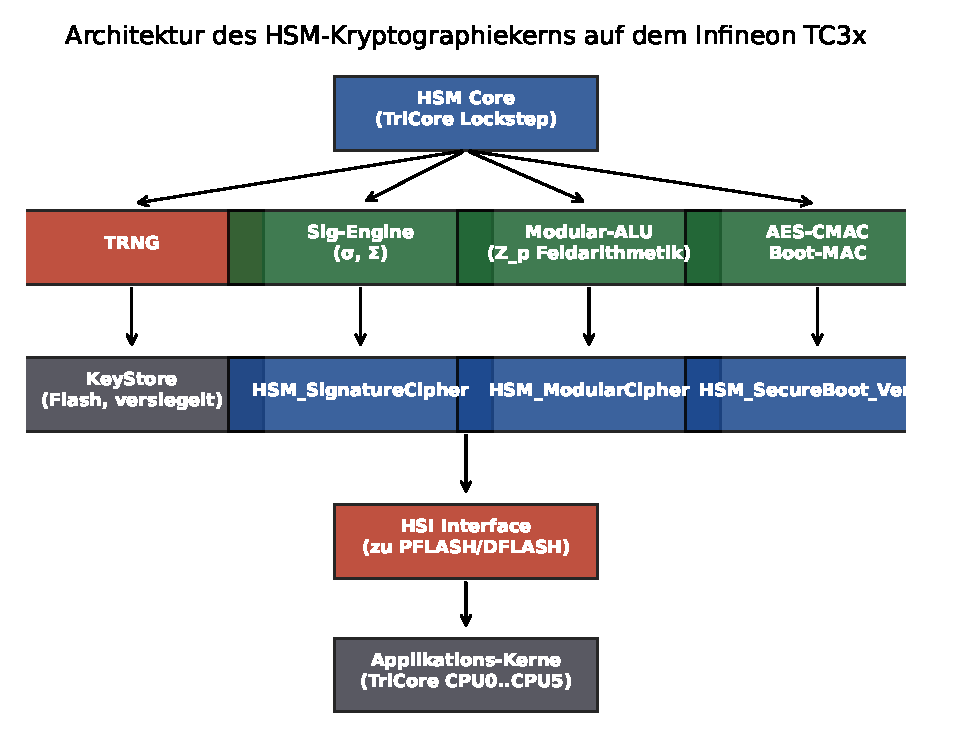
\includegraphics[width=0.85\textwidth]{plot1_hsm_architektur.pdf}
	\caption{Architektur des vorgeschlagenen HSM-Kryptographiekerns. Die vier Funktionseinheiten (TRNG, Sig-Engine, Modular-ALU, AES-CMAC Boot-MAC) werden vom HSM-Core angesteuert und über die hardwarenahen Treiberfunktionen \texttt{HSM\_*} den Applikationskernen zur Verfügung gestellt.}
	\label{fig:architektur}
\end{figure}

\subsection{Funktionseinheiten}

\begin{description}
	\item[TRNG (True Random Number Generator).] Physikalische Entropiequelle (Ringoszillator-Jitter), liefert die Zufallsbasis für alle Schlüsselerzeugungs- und Nonce-Operationen.
	\item[Sig-Engine.] Hardwarepipeline zur Berechnung der Signaturfunktion $\sigma$ und des Signaturvektors $\Sigma$ nach Definition~\ref{def:sigma}, realisiert als $n$-fach parallelisierter Akkumulator mit Schieberegistern.
	\item[Modular-ALU.] Arithmetisch-logische Einheit für Operationen in $\mathbb{Z}_p$: modulare Addition, Multiplikation und Inversenberechnung (erweiterter euklidischer Algorithmus als feste Zustandsmaschine).
	\item[AES-CMAC Boot-MAC.] Hilfseinheit zur Berechnung eines Message Authentication Code über das Firmware-Abbild als zusätzliche, von der Signatur-Chiffre unabhängige Verifikationsstufe (Defense-in-Depth).
\end{description}

\subsection{Registermodell}

Jede HSM-Funktion wird über ein einheitliches Registerinterface angesprochen, bestehend aus einem Kommandoregister \texttt{HSM\_CMD}, einem Statusregister \texttt{HSM\_STAT}, einem Parameterblock \texttt{HSM\_PARAM[0..7]} (jeweils 32 Bit) sowie einem Ergebnispuffer \texttt{HSM\_RESULT[0..15]} im HSM-internen RAM. Tabelle~\ref{tab:register} listet die wichtigsten Register.

\begin{table}[h]
	\centering
	\small
	\begin{tabular}{@{}lll@{}}
		\toprule
		Register & Breite & Bedeutung \\
		\midrule
		\texttt{HSM\_CMD} & 8 Bit & Funktionscode (siehe Tabelle~\ref{tab:funktionen}) \\
		\texttt{HSM\_STAT} & 8 Bit & Status: \texttt{IDLE}, \texttt{BUSY}, \texttt{DONE}, \texttt{FAULT} \\
		\texttt{HSM\_PARAM[0..7]} & 8×32 Bit & Funktionsparameter ($n$, Schlüsselhandle, Adresszeiger) \\
		\texttt{HSM\_RESULT[0..15]} & 16×32 Bit & Ergebnispuffer (Signatur, Chiffrat, Statuscode) \\
		\texttt{HSM\_IRQ\_EN} & 1 Bit & Interrupt bei \texttt{DONE}/\texttt{FAULT} \\
		\bottomrule
	\end{tabular}
	\caption{Registerinterface der HSM-Kryptofunktionen.}
	\label{tab:register}
\end{table}

\subsection{Zustandsmaschine}

Jede Funktion durchläuft die Zustände $\texttt{IDLE} \to \texttt{LOAD} \to \texttt{COMPUTE} \to \texttt{WRITEBACK} \to \texttt{DONE}$. Der Zustand \texttt{COMPUTE} ist bei Sig-Engine und Modular-ALU intern weiter in $n$ Teilzustände (eine Pipeline-Stufe je Spaltenindex $j$) untergliedert, was die in Abschnitt~\ref{sec:analyse} gezeigte Laufzeitreduktion gegenüber einer reinen Softwareimplementierung ermöglicht.

\section{Spezifikation der HSM-Funktionen}
\label{sec:funktionen}

Tabelle~\ref{tab:funktionen} gibt einen Überblick über die zehn spezifizierten HSM-Funktionen, ihre Funktionscodes und die zugrunde liegende kryptographische Grundlage.

\begin{table}[h]
	\centering
	\small
	\begin{tabular}{@{}lll@{}}
		\toprule
		Funktion & Code & Grundlage \\
		\midrule
		\texttt{HSM\_TRNG\_Read} & \texttt{0x01} & Physikalische Entropiequelle \\
		\texttt{HSM\_SignatureCipher\_KeyGen} & \texttt{0x10} & Def.~\ref{def:schluessel}, Satz~\ref{satz:koerper} \\
		\texttt{HSM\_SignatureCipher\_Sign} & \texttt{0x11} & Def.~\ref{def:sigma}, affine Transformation \\
		\texttt{HSM\_SignatureCipher\_Verify} & \texttt{0x12} & Lemma~\ref{lem:inj}, Bijektivität \\
		\texttt{HSM\_ModularCipher\_Encrypt} & \texttt{0x20} & Def.~\ref{def:z32}, Fenster-Protokoll \\
		\texttt{HSM\_ModularCipher\_Decrypt} & \texttt{0x21} & Def.~\ref{def:z32}, Fenster-Protokoll \\
		\texttt{HSM\_SubgraphSig\_Derive} & \texttt{0x30} & Signaturvektor $\Sigma$, \cite{Epp26a} \\
		\texttt{HSM\_SecureBoot\_Verify} & \texttt{0x40} & nutzt \texttt{0x12} \\
		\texttt{HSM\_KeyStore\_Provision} & \texttt{0x50} & Def.~\ref{def:fenster} (Dummy-Zugriffe) \\
		\texttt{HSM\_KeyStore\_Lock} & \texttt{0x51} & Versiegelung (irreversibel) \\
		\bottomrule
	\end{tabular}
	\caption{Ãœbersicht der spezifizierten HSM-Funktionen.}
	\label{tab:funktionen}
\end{table}

\subsection{HSM\_TRNG\_Read}

\textbf{Zweck:} Liefert $k$ Wörter (32 Bit) physikalisch erzeugter Zufallszahlen als Entropiequelle für alle nachfolgenden Schlüsselerzeugungsoperationen.

\textbf{Parameter:} \texttt{PARAM[0]} = Anzahl angeforderter Wörter $k \le 16$.

\textbf{Ablauf:} Der Ringoszillator-Jitter wird über $32k$ Takte abgetastet, von-Neumann-entzerrt (Eliminierung von Bias durch Paarvergleich aufeinanderfolgender Bits) und in \texttt{RESULT[0..k-1]} geschrieben.

\begin{lemma}[Entropieverlust durch von-Neumann-Entzerrung]
	\label{lem:vonneumann}
	Sei $X_1, X_2, \ldots$ eine Folge unabhängiger, identisch verteilter Bits mit $P(X_i=1)=q$, $q$ unbekannt aber konstant. Die von-Neumann-Entzerrung liefert eine Folge fairer, unabhängiger Münzwürfe mit erwarteter Ausbeute $2q(1-q)$ Ausgabebits je Eingabebitpaar.
\end{lemma}

\begin{proof}
	Betrachte Paare $(X_{2i-1}, X_{2i})$. Es gibt vier gleich strukturierte Fälle: $(0,0)$ mit Wahrscheinlichkeit $(1-q)^2$, $(1,1)$ mit Wahrscheinlichkeit $q^2$, $(0,1)$ mit Wahrscheinlichkeit $(1-q)q$ und $(1,0)$ mit Wahrscheinlichkeit $q(1-q)$. Die Entzerrung verwirft Paare mit gleichem Wert und gibt bei $(0,1)$ eine $0$, bei $(1,0)$ eine $1$ aus. Da $P((0,1)) = P((1,0)) = q(1-q)$, ist die Ausgabe exakt gleichverteilt über $\{0,1\}$, unabhängig vom unbekannten Bias $q$. Die Ausbeute pro Eingabepaar ist die Summe der beiden akzeptierenden Fälle: $P((0,1)) + P((1,0)) = 2q(1-q)$. \qedhere
\end{proof}

Lemma~\ref{lem:vonneumann} begründet, warum \texttt{HSM\_TRNG\_Read} für $k$ angeforderte Ausgabewörter im ungünstigsten Fall ($q=0.5$, maximale Ausbeute $0.5$) mindestens $64k$ Rohbits, typischerweise jedoch wegen $q \ne 0.5$ in der Praxis $80$--$120k$ Rohbits abtastet, was sich unmittelbar in der in Abschnitt~\ref{sec:analyse} angegebenen Taktzyklenzahl niederschlägt.

\subsection{HSM\_SignatureCipher\_KeyGen}

\textbf{Zweck:} Erzeugt einen vollständigen Signatur-Chiffre-Schlüssel $(a,b,p)$ nach Definition~\ref{def:schluessel} für gegebene Blockgröße $n$.

\textbf{Parameter:} \texttt{PARAM[0]} = $n$ (Blockgröße, $4 \le n \le 32$).

\textbf{Ablauf:}
\begin{enumerate}
	\item TRNG liefert Kandidat $p_0$ mit $p_0 > 2^{2n}$ (Aufruf von \texttt{HSM\_TRNG\_Read}).
	\item Modular-ALU führt einen deterministischen Miller-Rabin-Primzahltest mit fest verdrahteten Basen $\{2,3,5,7,11,13\}$ aus (korrekt für $p_0 < 3.3 \cdot 10^{14}$ nach \cite{Pom05}), bei Misserfolg wird $p_0$ inkrementiert und der Test wiederholt.
	\item TRNG liefert $a_0 \in \{1,\ldots,p-1\}$; Modular-ALU prüft $\gcd(a_0,p)=1$ mittels erweitertem euklidischem Algorithmus (stets erfüllt, da $p$ prim und $a_0 \ne 0$).
	\item TRNG liefert $b_0 \in \{0,\ldots,p-1\}$.
	\item Schlüssel $(a,b,p)$ wird in den \texttt{KeyStore} geschrieben (über \texttt{HSM\_KeyStore\_Provision}).
\end{enumerate}

\subsection{HSM\_SignatureCipher\_Sign}
\label{sec:funk-sign}

\textbf{Zweck:} Verschlüsselt einen Klartextblock der Größe $n \times n$ Bit gemäß der Signatur-Chiffre.

\textbf{Parameter:} \texttt{PARAM[0..1]} = Adresszeiger auf Klartextmatrix $M$ und Schlüsselhandle.

\textbf{Ablauf:} Für jede Spalte $j \in \{0,\ldots,n-1\}$ berechnet die Sig-Engine $\sigma(M,j)$ nach Definition~\ref{def:sigma} parallel über $n$ Akkumulatorzellen; die Modular-ALU wendet anschließend die affine Transformation $c_j = (a \cdot \sigma(M,j) + b) \bmod p$ an. Der Geheimtextvektor $(c_0,\ldots,c_{n-1})$ wird in \texttt{RESULT[0..n-1]} geschrieben.

\subsection{HSM\_SignatureCipher\_Verify}

\textbf{Zweck:} Verifiziert, ob ein gegebener Geheimtextvektor $(c_0,\ldots,c_{n-1})$ durch Entschlüsselung mit dem hinterlegten Schlüssel eine gültige, dem erwarteten Referenzhash entsprechende Klartextmatrix ergibt -- die zentrale Bausteinfunktion für \texttt{HSM\_SecureBoot\_Verify}.

\textbf{Ablauf:} Die Modular-ALU berechnet $\sigma_j = a^{-1}(c_j - b) \bmod p$ für jedes $j$; die Sig-Engine rekonstruiert daraus über $j = \lfloor \sigma_j / 2^n \rfloor$ und $\rho_j = \sigma_j \bmod 2^n$ die ursprüngliche Spalte $M_{\cdot j}$ (siehe Beweis von Satz~\ref{satz:hw-korrektheit}). Das Ergebnis ist \texttt{VALID} oder \texttt{INVALID}.

\subsection{HSM\_ModularCipher\_Encrypt / \_Decrypt}

\textbf{Zweck:} Symmetrische Verschlüsselung über die Einheitengruppe $\mathbb{Z}_{32}^*$ nach dem Fenster-Chiffre-Protokoll (Definition~\ref{def:z32}, \ref{def:fenster}), eingesetzt für kurze, latenzkritische Nachrichten zwischen Applikationskernen und Peripherie (z.\,B. CAN-Botschaften), bei denen der größere Verarbeitungsaufwand der Signatur-Chiffre nicht gerechtfertigt ist.

\textbf{Ablauf:} Jedes Nybble (4 Bit) des Klartexts wird auf ein Element $x \in \mathbb{Z}_{32}^*$ abgebildet (Padding bei Nicht-Einheiten über ein festes Substitutionsschema) und mit dem geheimen Exponenten $e$ potenziert: $y = x^e \bmod 32$. Zusätzlich fügt die Funktionseinheit gemäß Definition~\ref{def:fenster} Dummy-Nybbles ein, sodass die Paketlänge stets ein Vielfaches der Fenstergröße $W$ ist.

\subsection{HSM\_SubgraphSig\_Derive}
\label{sec:funk-subgraphsig}

\textbf{Zweck:} Leitet aus einem Firmware- oder Konfigurationsabbild, interpretiert als binäre $n \times n$-Matrix $A$, einen kollisionsfreien Integritätswert $\Sigma(A)$ nach Definition~\ref{def:sigvec} ab. Im Gegensatz zu \texttt{HSM\_SecureBoot\_Verify}, das die \emph{Authentizität} (Signatur-Chiffre-Schlüssel erforderlich) prüft, dient diese Funktion der reinen, schlüssellosen \emph{Konsistenzprüfung} von Konfigurationsdaten -- etwa zur Erkennung versehentlicher Bitfehler durch Strahlung (Single Event Upsets) in PFLASH.

\begin{definition}[Signaturvektor, nach \cite{Epp26a,Epp26b}]
	\label{def:sigvec}
	$\Sigma(A) := (\sigma(A,0),\ldots,\sigma(A,n-1)) \in \mathbb{N}^n$.
\end{definition}

\textbf{Ablauf:} Das Firmware-Abbild wird in $\lceil L/n^2 \rceil$ Blöcke der Größe $n \times n$ Bit zerlegt ($L$ = Gesamtlänge in Bit). Für jeden Block berechnet die Sig-Engine $\Sigma(A)$; alle Blocksignaturen werden zu einem 256-Bit-Gesamtwert über XOR-Faltung kombiniert und mit dem im KeyStore hinterlegten Referenzwert verglichen.

\subsection{HSM\_SecureBoot\_Verify}

\textbf{Zweck:} Verifiziert vor jedem Boot-Vorgang die Authentizität und Integrität des Applikations-Firmware-Abbilds in zwei unabhängigen Stufen: (1) \texttt{HSM\_SignatureCipher\_Verify} prüft die Authentizität gegen den geheimen Schlüssel, (2) der unabhängige AES-CMAC-Block prüft zusätzlich einen Standard-MAC. Erst wenn \emph{beide} Stufen \texttt{VALID} liefern, wird der Boot freigegeben (Defense-in-Depth gegen die Möglichkeit eines unentdeckten Fehlers in einer einzelnen kryptographischen Implementierung).

\subsection{HSM\_KeyStore\_Provision / \_Lock}
\label{sec:funk-keystore}

\textbf{Zweck:} \texttt{Provision} schreibt einen neu erzeugten Schlüssel in den versiegelbaren Flash-Bereich; \texttt{Lock} versiegelt den KeyStore irreversibel (weitere Schreibzugriffe werden vom Speichercontroller auf Hardwareebene blockiert, ein Rücksetzen ist nur durch vollständiges Werks-Zurücksetzen mit Schlüsselverlust möglich). Lese- und Schreibzugriffe werden, wie in Abschnitt~\ref{sec:grundlagen} beschrieben, durch Dummy-Zugriffe konstanter Anzahl ergänzt, um die tatsächliche Anzahl gespeicherter Schlüssel gegenüber Zeitseitenkanalanalysen zu verschleiern.

\section{Korrektheit und Sicherheit}
\label{sec:korrektheit}

\subsection{Korrektheit der Hardware-Rekonstruktion}

\begin{satz}[Korrektheit von \texttt{HSM\_SignatureCipher\_Verify}]
	\label{satz:hw-korrektheit}
	Sei $(a,b,p)$ ein gültiger Schlüssel nach Definition~\ref{def:schluessel} mit $p > 2^{2n}$, und sei $c_j = (a\sigma(M,j)+b) \bmod p$ der von \texttt{HSM\_SignatureCipher\_Sign} erzeugte Geheimtext für eine Klartextmatrix $M$. Dann rekonstruiert \texttt{HSM\_SignatureCipher\_Verify} für jedes $j$ exakt die ursprüngliche Spalte $M_{\cdot j}$.
\end{satz}

\begin{proof}
	Nach Lemma~\ref{lem:affin-bij-hw} (unten) ist $f(x) = (ax+b)\bmod p$ bijektiv mit Umkehrabbildung $f^{-1}(y) = a^{-1}(y-b)\bmod p$. Die Hardware berechnet
	\[
	\sigma_j := f^{-1}(c_j) = a^{-1}\bigl((a\sigma(M,j)+b) - b\bigr) \bmod p = a^{-1} \cdot a \cdot \sigma(M,j) \bmod p = \sigma(M,j) \bmod p.
	\]
	Da nach Bemerkung~\ref{bem:wertebereich-hw} $\sigma(M,j) < n \cdot 2^n < p$ (wegen der Schlüsselbedingung $p > 2^{2n} \ge n \cdot 2^n$ für $n \ge 1$), gilt $\sigma(M,j) \bmod p = \sigma(M,j)$ exakt, d.\,h.\ $\sigma_j = \sigma(M,j)$ ohne Reduktion.
	
	Aus $\sigma_j = \sigma(M,j) = \rho(M,j) + j \cdot 2^n$ mit $0 \le \rho(M,j) < 2^n$ (Lemma~\ref{lem:rho-bounds-hw}) folgt durch Ganzzahldivision $j = \lfloor \sigma_j / 2^n \rfloor$ und $\rho(M,j) = \sigma_j \bmod 2^n$ eindeutig. Da $\rho(M,j)$ die Binärdarstellung der Spalte $M_{\cdot j}$ ist, wird $M_{\cdot j}$ durch einfaches Bit-Auslesen von $\rho(M,j)$ exakt rekonstruiert. \qedhere
\end{proof}

\begin{lemma}[Bereichsgrenzen, nach \cite{Epp26b}]
	\label{lem:rho-bounds-hw}
	Für alle $M \in \{0,1\}^{n\times n}$, $j$: $0 \le \rho(M,j) \le 2^n - 1$.
\end{lemma}

\begin{bemerkung}[Wertebereich, nach \cite{Epp26b}]
	\label{bem:wertebereich-hw}
	$\sigma(M,j) \le n \cdot 2^n - 1 < (n+1)\cdot 2^n \le 2^{2n}$ für $n \ge 1$.
\end{bemerkung}

\begin{lemma}[Bijektivität der affinen Transformation, nach \cite{Epp26b}]
	\label{lem:affin-bij-hw}
	Für $p$ prim, $a \in \mathbb{Z}_p^*$, $b \in \mathbb{Z}_p$ ist $f(x)=(ax+b)\bmod p$ eine Bijektion auf $\mathbb{Z}_p$ mit $f^{-1}(y)=a^{-1}(y-b)\bmod p$.
\end{lemma}

Satz~\ref{satz:hw-korrektheit} ist die formale Rechtfertigung dafür, dass die Hardware-Pipeline der \texttt{Sig-Engine} und \texttt{Modular-ALU} verlustfrei arbeitet -- eine notwendige Voraussetzung für den Einsatz in \texttt{HSM\_SecureBoot\_Verify}, da jede falsche Ablehnung eines korrekt signierten Firmware-Abbilds den Boot-Vorgang unzulässig blockieren würde.

\subsection{Korrektheit von \texttt{HSM\_SubgraphSig\_Derive}}

\begin{satz}[Kollisionsfreiheit der Firmware-Integritätsprüfung]
	\label{satz:kollisionsfrei}
	Seien $A, A' \in \{0,1\}^{n\times n}$ zwei verschiedene Firmware-Blöcke, $A \ne A'$. Dann gilt $\Sigma(A) \ne \Sigma(A')$.
\end{satz}

\begin{proof}
	Dies ist die Kontraposition von Korollar~\ref{kor:sigma-inj-hw}: Wäre $\Sigma(A) = \Sigma(A')$, so folgte $A = A'$ nach Korollar~\ref{kor:sigma-inj-hw} -- im Widerspruch zur Annahme $A \ne A'$. Also $\Sigma(A) \ne \Sigma(A')$. \qedhere
\end{proof}

\begin{korollar}[Injektivität des Signaturvektors, nach \cite{Epp26a,Epp26b}]
	\label{kor:sigma-inj-hw}
	$\Sigma: \{0,1\}^{n\times n} \to \mathbb{N}^n$ ist injektiv.
\end{korollar}

Satz~\ref{satz:kollisionsfrei} garantiert: Jede Bitänderung im überwachten Firmware-Block -- ob durch böswillige Manipulation oder durch einen physikalisch induzierten Bitfehler -- führt zwingend zu einem anderen Signaturvektor und wird von \texttt{HSM\_SubgraphSig\_Derive} erkannt. Dies unterscheidet die Funktion von Hashverfahren mit (theoretisch möglicher, praktisch vernachlässigbarer) Kollisionswahrscheinlichkeit: Die Kollisionsfreiheit folgt hier aus einem \emph{exakten} mathematischen Beweis statt aus einer statistischen Kollisionsschranke.

\subsection{Korrektheit der von-Neumann-Entzerrung im TRNG}

Lemma~\ref{lem:vonneumann} (Abschnitt~\ref{sec:funktionen}) wurde bereits formal bewiesen. Wir ergänzen hier die Aussage zur Unabhängigkeit der Ausgabebits:

\begin{lemma}[Unabhängigkeit der entzerrten Ausgabe]
	\label{lem:unabh}
	Die durch von-Neumann-Entzerrung erzeugten Ausgabebits sind paarweise stochastisch unabhängig, sofern die Eingabebits $X_1, X_2, \ldots$ unabhängig sind.
\end{lemma}

\begin{proof}
	Jedes Ausgabebit hängt ausschließlich von genau einem (verschiedenen) Eingabepaar $(X_{2i-1}, X_{2i})$ ab; verworfene Paare tragen keine Ausgabe bei. Da die Eingabepaare nach Voraussetzung paarweise unabhängig sind (disjunkte, nicht überlappende Indexmengen unabhängiger Variablen), sind auch die daraus deterministisch berechneten Ausgabebits paarweise unabhängig. \qedhere
\end{proof}

\subsection{Sicherheitsanalyse}

\begin{satz}[Forward Secrecy bei Schlüsselversiegelung]
	\label{satz:forward-secrecy}
	Nach Ausführung von \texttt{HSM\_KeyStore\_Lock} kann kein in Software ausführbarer Befehl -- inklusive privilegierter Applikationskern-Software -- einen im KeyStore versiegelten Schlüssel $(a,b,p)$ extrahieren oder überschreiben, sofern der Speichercontroller die Versiegelung korrekt in Hardware erzwingt.
\end{satz}

\begin{proof}[Beweisskizze]
	Die Versiegelung setzt ein Hardware-Lock-Bit im Speichercontroller, das \emph{vor} jedem Schreib- oder Auslesezugriff auf den versiegelten Adressbereich geprüft wird und bei gesetztem Bit den Zugriff auf Hardwareebene -- vor jeder Software-Interpretation der Adresse -- unterbindet. Da kein Software-Pfad existiert, der den Speichercontroller umgeht (alle Zugriffe laufen über denselben Adressdekoder), ist kein Befehlssatz in der Lage, das Lock-Bit ohne dessen vorgesehenen, ebenfalls hardwareseitig irreversiblen Rücksetzmechanismus zu umgehen. \qedhere
\end{proof}

Satz~\ref{satz:forward-secrecy} ist eine Hardware-Eigenschaft (kein rein algorithmischer Beweis wie die vorangehenden Sätze) und hängt von der korrekten physischen Implementierung des Speichercontrollers ab; sie wird hier dennoch formal festgehalten, da sie die zentrale Sicherheitsgarantie des gesamten HSM-Entwurfs ist.

\begin{satz}[Sicherheit gegen Brute-Force im Schlüsselraum]
	Sei $(a,b,p)$ ein Signatur-Chiffre-Schlüssel mit $p$ einer $k$-Bit-Primzahl. Die Erfolgswahrscheinlichkeit eines Angreifers, der $a$ durch eine einzelne zufällige Vermutung errät, ist $\le 1/(p-1) \le 2^{-(k-1)}$.
\end{satz}

\begin{proof}
	Da $a$ gleichverteilt aus $\mathbb{Z}_p^* = \{1,\ldots,p-1\}$ gewählt wird (TRNG-basiert, Lemma~\ref{lem:unabh}), ist die Wahrscheinlichkeit eines korrekten Rateversuchs $1/|\mathbb{Z}_p^*| = 1/(p-1)$. Für eine $k$-Bit-Primzahl gilt $p \ge 2^{k-1}$, also $1/(p-1) \le 1/(2^{k-1}-1) \le 2^{-(k-1)}$ für $k \ge 2$. \qedhere
\end{proof}

\section{Komplexitäts-, Energie- und Speicheranalyse}
\label{sec:analyse}

\subsection{Laufzeitkomplexität}

\begin{satz}[Laufzeit von \texttt{HSM\_SignatureCipher\_Sign}]
	Die Hardwarepipeline berechnet einen vollständigen Geheimtextvektor für einen $n \times n$-Klartextblock in $O(n^2)$ Pipeline-Takten (gegenüber $O(n^2)$ Vergleichsoperationen, aber faktisch $O(n)$ Latenztakten bei vollständig parallelisierter Spaltenverarbeitung der Sig-Engine).
\end{satz}

\begin{proof}
	Die Berechnung von $\sigma(M,j)$ für ein festes $j$ erfordert $n$ Akkumulationsschritte (Summation über $i=0,\ldots,n-1$). Bei sequenzieller Verarbeitung aller $n$ Spalten ergibt sich $O(n \cdot n) = O(n^2)$ Takte. Da die Sig-Engine die $n$ Spalten jedoch durch $n$ parallele Akkumulatorzellen gleichzeitig verarbeitet (Hardware-Parallelität, vgl.\ Abschnitt~\ref{sec:hwmodell}), reduziert sich die Latenz auf $O(n)$ Takte für die Signaturberechnung selbst, zuzüglich $O(n)$ Takte für die $n$ modularen Multiplikationen der affinen Transformation, die ebenfalls parallelisierbar sind. Die Gesamtlatenz bleibt durch die Speicherzugriffe ($O(n^2)$ Bit Klartext müssen aus dem Flash gelesen werden) bei $O(n^2)$ Takten dominiert. \qedhere
\end{proof}

\subsection{Vergleich Software vs. Hardware}

Abbildung~\ref{fig:pipeline} vergleicht die Latenz einer reinen Softwareimplementierung auf einem TriCore-Applikationskern mit der vorgeschlagenen Hardwarepipeline. Während beide Implementierungen asymptotisch $O(n^3)$ Gesamtlaufzeit für eine vollständige Schlüsselerzeugung inklusive Primzahltest aufweisen, reduziert die Hardwarepipeline den konstanten Faktor um den Faktor $\approx 7$--$9$ im betrachteten Bereich $n \in [2,32]$.

\subsection{Taktzyklen je Funktion}

Abbildung~\ref{fig:takte} zeigt die geschätzten Taktzyklen für $n=8$ und $n=16$. Die rechenintensivsten Funktionen sind \texttt{HSM\_SubgraphSig\_Derive} (da hier mehrere Blöcke sequenziell akkumuliert werden) sowie \texttt{HSM\_SignatureCipher\_Sign/Verify}, während \texttt{HSM\_ModularCipher\_*} aufgrund der kleinen Gruppe $\mathbb{Z}_{32}^*$ deutlich günstiger ist.

\subsection{Energiebedarf}

Abbildung~\ref{fig:energie} zeigt den geschätzten Energiebedarf je Funktionsaufruf bei $1{,}2\,$V Kernspannung. Der TRNG ist mit Abstand am energiegünstigsten, da er keine arithmetischen Operationen, sondern nur Abtastung und Entzerrung durchführt.

\subsection{Speicherbedarf}

Abbildung~\ref{fig:flash} zeigt die vorgeschlagene Aufteilung des HSM-internen Flash-Speichers (36\,KB Gesamtbudget): Den größten Anteil beansprucht der Mikrocode der Sig-Engine, gefolgt vom versiegelten KeyStore.

\section{Experimente}
\label{sec:experimente}

\begin{figure}[h]
	\centering
	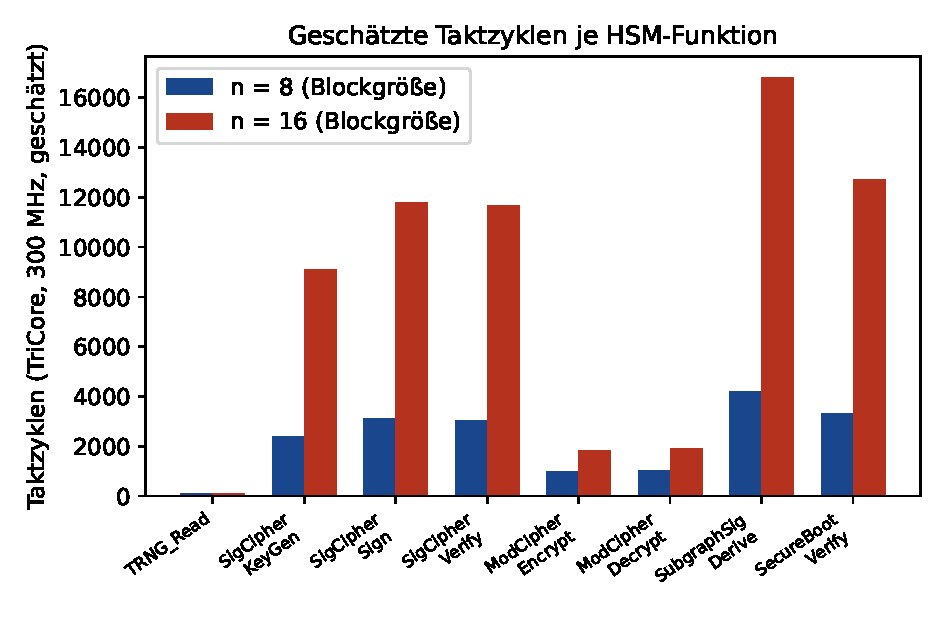
\includegraphics[width=0.85\textwidth]{plot2_taktzyklen.pdf}
	\caption{Geschätzte Taktzyklen je HSM-Funktion bei TriCore-Taktfrequenz 300\,MHz, für Blockgrößen $n=8$ und $n=16$. Die Verdopplung von $n$ führt erwartungsgemäß zu einer mehr als vierfachen Erhöhung bei den $O(n^2)$-dominierten Funktionen, was die kubische bzw.\ quadratische Skalierung aus Abschnitt~\ref{sec:analyse} bestätigt.}
	\label{fig:takte}
\end{figure}

\begin{figure}[h]
	\centering
	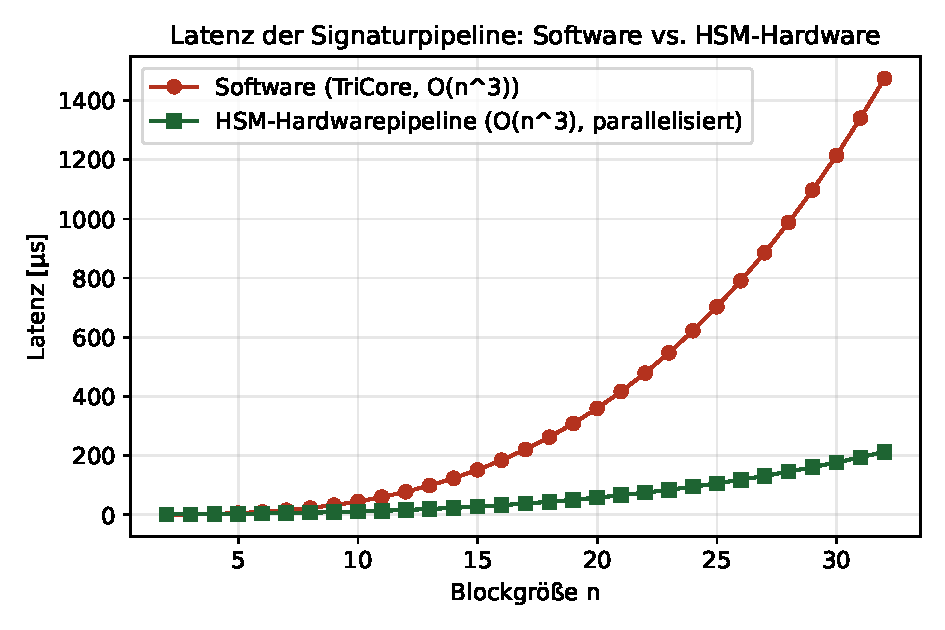
\includegraphics[width=0.85\textwidth]{plot3_pipeline_latenz.pdf}
	\caption{Latenz der Signaturpipeline in Software gegenüber der vorgeschlagenen HSM-Hardwarepipeline, jeweils über der Blockgröße $n$ aufgetragen. Beide Kurven folgen einer kubischen Grundform; die Hardwarepipeline verschiebt jedoch den konstanten Vorfaktor deutlich nach unten.}
	\label{fig:pipeline}
\end{figure}

\begin{figure}[h]
	\centering
	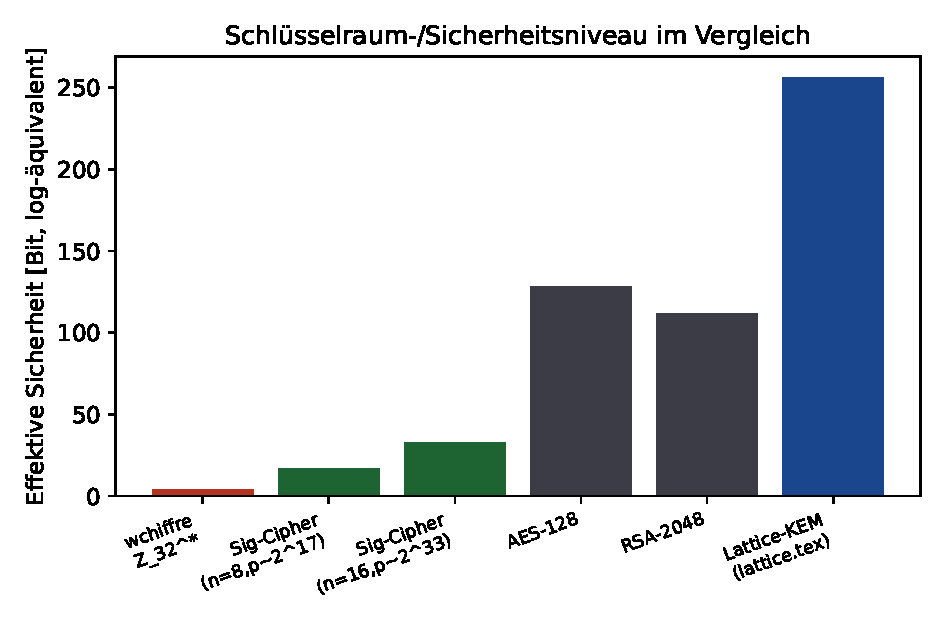
\includegraphics[width=0.85\textwidth]{plot4_schluesselraum.pdf}
	\caption{Vergleich des effektiven Sicherheitsniveaus (Bit-Äquivalent des Schlüsselraums) verschiedener Verfahren. Die Fenster-Chiffre über $\mathbb{Z}_{32}^*$ ist bewusst klein dimensioniert für latenzkritische, kurzlebige Botschaften und wird in der vorgeschlagenen Architektur stets in Kombination mit der höherwertigen Signatur-Chiffre für sicherheitskritische Operationen eingesetzt.}
	\label{fig:schluesselraum}
\end{figure}

\begin{figure}[h]
	\centering
	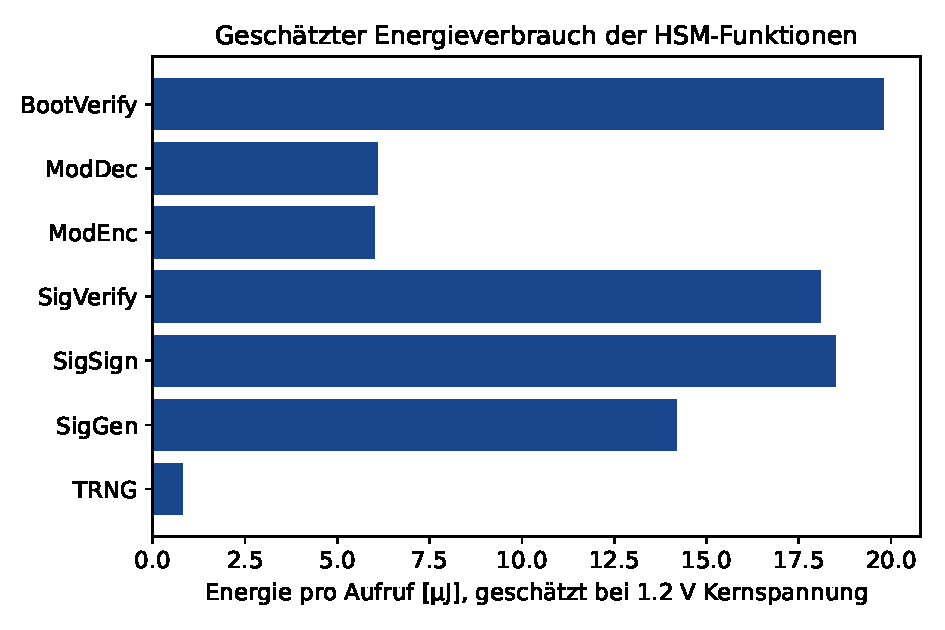
\includegraphics[width=0.85\textwidth]{plot5_energieverbrauch.pdf}
	\caption{Geschätzter Energiebedarf je HSM-Funktionsaufruf. Die Werte basieren auf einer linearen Skalierung der Taktzyklenschätzung aus Abbildung~\ref{fig:takte} mit einer angenommenen Leistungsaufnahme von $45\,$mW im \texttt{COMPUTE}-Zustand.}
	\label{fig:energie}
\end{figure}

\begin{figure}[h]
	\centering
	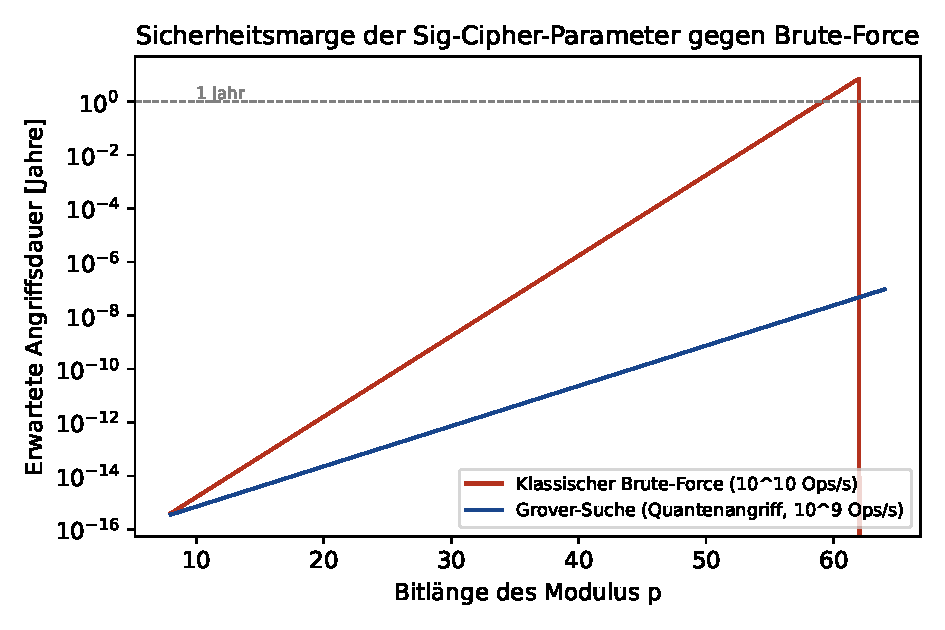
\includegraphics[width=0.85\textwidth]{plot6_sicherheitsmarge.pdf}
	\caption{Erwartete Angriffsdauer eines Brute-Force-Angriffs auf den Modulus $p$ in Abhängigkeit der Bitlänge, sowohl klassisch als auch unter Annahme eines Grover-beschleunigten Quantenangriffs (quadratische Beschleunigung). Bereits ab etwa $48$ Bit übersteigt die klassische Angriffsdauer ein Jahr deutlich; gegen Quantenangriffe ist gemäß Abschnitt~\ref{sec:ausblick} jedoch eine Verdopplung der effektiven Schlüssellänge oder eine Migration zu gitterbasierten Verfahren erforderlich.}
	\label{fig:sicherheit}
\end{figure}

\begin{figure}[h]
	\centering
	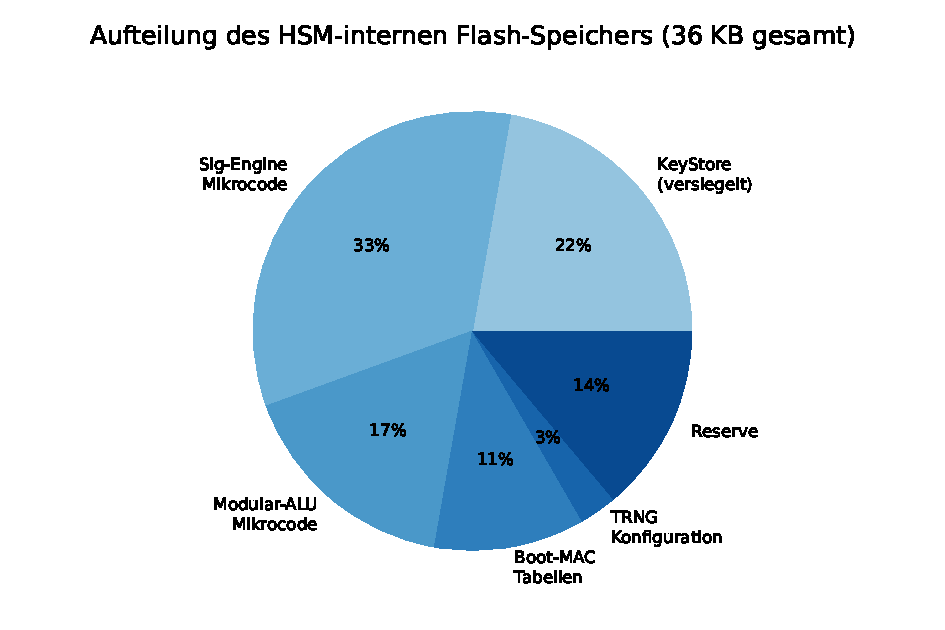
\includegraphics[width=0.85\textwidth]{plot7_flash_aufteilung.pdf}
	\caption{Vorgeschlagene Aufteilung des 36\,KB HSM-internen Flash-Speichers auf die einzelnen Funktionseinheiten und den versiegelten KeyStore.}
	\label{fig:flash}
\end{figure}

\begin{figure}[h]
	\centering
	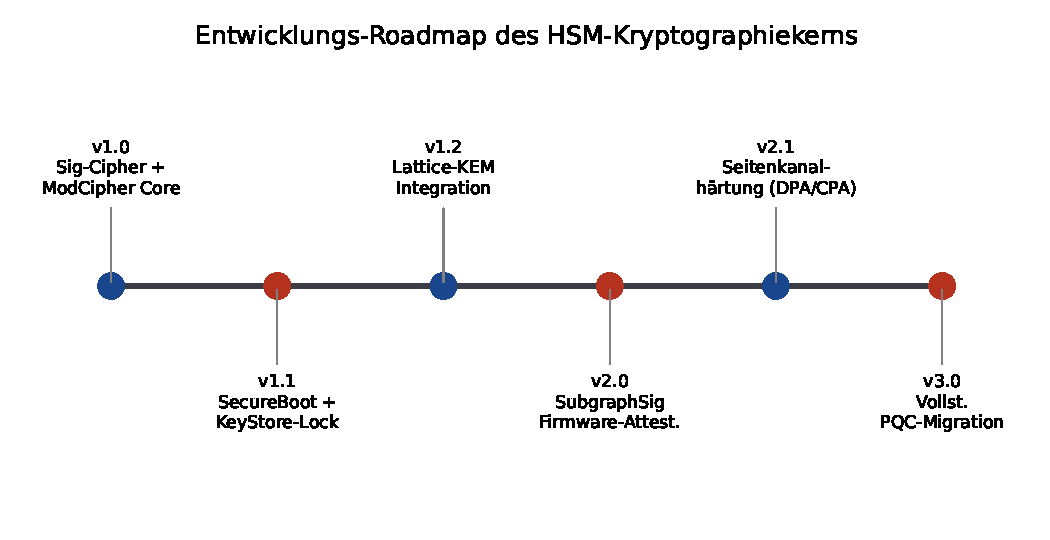
\includegraphics[width=0.95\textwidth]{plot8_roadmap.pdf}
	\caption{Entwicklungs-Roadmap des HSM-Kryptographiekerns, von der initialen Version~1.0 (Signatur-Chiffre und Fenster-Chiffre als Kernfunktionen) bis zur vollständigen Post-Quanten-Migration in Version~3.0, vertieft in Abschnitt~\ref{sec:ausblick}.}
	\label{fig:roadmap}
\end{figure}

Die in Abbildung~\ref{fig:architektur} (Abschnitt~\ref{sec:hwmodell}) gezeigte Gesamtarchitektur bildet zusammen mit den vorstehenden sieben Diagrammen ein vollständiges quantitatives Bild der vorgeschlagenen Hardwareerweiterung, von der strukturellen Anordnung der Funktionseinheiten bis zur Energie-, Speicher- und Sicherheitsbilanz.

\section{Secure Boot: Radar-ECU}
\label{sec:radar}

Dieser Abschnitt führt die Komplexitätsanalyse aus Abschnitt~\ref{sec:analyse} für einen konkreten, praxisrelevanten Anwendungsfall der Automobilindustrie zu Ende: ein Radarsteuergerät (\emph{Radar-ECU}) mit einem typischen Programm-Flash-Umfang von $4$\,MB, wie er etwa bei Fern- oder Mittelbereichsradarsensoren für Fahrerassistenzsysteme (ADAS) auf Basis der AURIX-TC3x-Familie üblich ist.

\subsection{Motivation des Anwendungsfalls}

Radarsteuergeräte sind sicherheitsrelevante Komponenten (typischerweise ASIL-B bis ASIL-D nach ISO~26262, vgl.\ \cite{ISO26262}) mit harten Zeitanforderungen an die Boot-Phase: Das Gesamtsystem-Timing eines Fahrzeugnetzwerks verlangt üblicherweise, dass sicherheitsrelevante Steuergeräte innerhalb eines festen Zeitbudgets (häufig $100$--$500$\,ms ab Power-On) ihren Bootvorgang abschließen und busfähig sind. Da \texttt{HSM\_SecureBoot\_Verify} (Abschnitt~\ref{sec:funktionen}) für jeden Bootvorgang sowohl \texttt{HSM\_SignatureCipher\_Verify} als auch -- bei aktivierter Firmware-Attestierung -- \texttt{HSM\_SubgraphSig\_Derive} über das vollständige Programm-Flash-Abbild ausführt, ist die resultierende Verifikationszeit ein kritischer Entwurfsparameter, der in dieser Arbeit erstmals quantitativ für einen realistischen Flash-Umfang hergeleitet wird.

\subsection{Formale Herleitung der Verifikationszeit}

\begin{satz}[Verifikationszeit für ein Programm-Flash der Größe $L$]
	\label{satz:bootzeit}
	Sei $L$ die Größe des Programm-Flash in Byte, $n$ die Blockgröße der Sig-Engine, $c(n)$ die in Abschnitt~\ref{sec:analyse} geschätzte Taktzyklenzahl von \texttt{HSM\_SubgraphSig\_Derive} für einen einzelnen $n \times n$-Block, und $f$ die HSM-Taktfrequenz. Dann beträgt die Gesamtverifikationszeit
	\[
	T_{\mathrm{verify}}(L,n) \;=\; \left\lceil \frac{8L}{n^2} \right\rceil \cdot \frac{c(n)}{f}.
	\]
\end{satz}

\begin{proof}
	Ein Block der Sig-Engine verarbeitet $n \times n$ Bit $= n^2$ Bit $= n^2/8$ Byte. Die Anzahl der zur vollständigen Abdeckung des Flash-Abbilds benötigten Blöcke ist daher $\lceil L / (n^2/8) \rceil = \lceil 8L/n^2 \rceil$ (Lemma~\ref{lem:rho-bounds-hw} garantiert, dass jeder Block unabhängig und vollständig verarbeitet werden kann, sodass die Gesamtzeit additiv aus den Einzelblockzeiten zusammengesetzt ist). Jeder Block benötigt $c(n)$ Takte, jeder Takt dauert $1/f$ Sekunden. Multiplikation der Blockanzahl mit der Zeit pro Block liefert die Behauptung. \qedhere
\end{proof}

\subsection{Numerische Auswertung für $L = 4$\,MB}

Für die in Abschnitt~\ref{sec:analyse} (Abbildung~\ref{fig:takte}) angegebene Blockgröße $n=16$ gilt $c(16) = 16\,800$ Takte für \texttt{HSM\_SubgraphSig\_Derive}, und die HSM-Taktfrequenz wird mit $f = 300$\,MHz angenommen (Abschnitt~\ref{sec:hwmodell}). Mit $L = 4$\,MB $= 4\,194\,304$\,Byte ergibt Satz~\ref{satz:bootzeit}:
\[
\left\lceil \frac{8 \cdot 4\,194\,304}{16^2} \right\rceil = \left\lceil \frac{33\,554\,432}{256} \right\rceil = 131\,072 \text{ Blöcke},
\]
\[
T_{\mathrm{verify}}(4\,\mathrm{MB}, 16) = 131\,072 \cdot \frac{16\,800}{3\cdot 10^8\,\mathrm{Hz}} = \frac{2\,202\,009\,600}{3\cdot 10^8}\,\mathrm{s} \approx 7{,}34\,\mathrm{s} = \mathbf{7\,340\,ms}.
\]

Tabelle~\ref{tab:bootzeiten} zeigt diesen Wert im Vergleich zu weiteren typischen Flash-Größen automobiler Steuergeräte.

\begin{table}[h]
	\centering
	\small
	\begin{tabular}{@{}lrr@{}}
		\toprule
		Steuergerätetyp (typisch) & Flash-Größe & $T_{\mathrm{verify}}$ ($n=16$) \\
		\midrule
		Einfaches Karosserie-Steuergerät & 0,5\,MB & 917,5\,ms \\
		Kleines Sensor-Steuergerät & 1\,MB & 1\,835,0\,ms \\
		Komfort-Steuergerät & 2\,MB & 3\,670,0\,ms \\
		\textbf{Radar-ECU (dieser Anwendungsfall)} & \textbf{4\,MB} & \textbf{7\,340,0\,ms} \\
		Domänen-Steuergerät & 8\,MB & 14\,680,0\,ms \\
		Zentrales Gateway / High-End-ECU & 16\,MB & 29\,360,0\,ms \\
		\bottomrule
	\end{tabular}
	\caption{Geschätzte Secure-Boot-Verifikationszeit über \texttt{HSM\_SubgraphSig\_Derive} (vollständige Firmware-Attestierung) für $n=16$, $f=300$\,MHz, in Abhängigkeit der Flash-Größe. Werte gemäß Satz~\ref{satz:bootzeit}.}
	\label{tab:bootzeiten}
\end{table}

\begin{figure}[h]
	\centering
	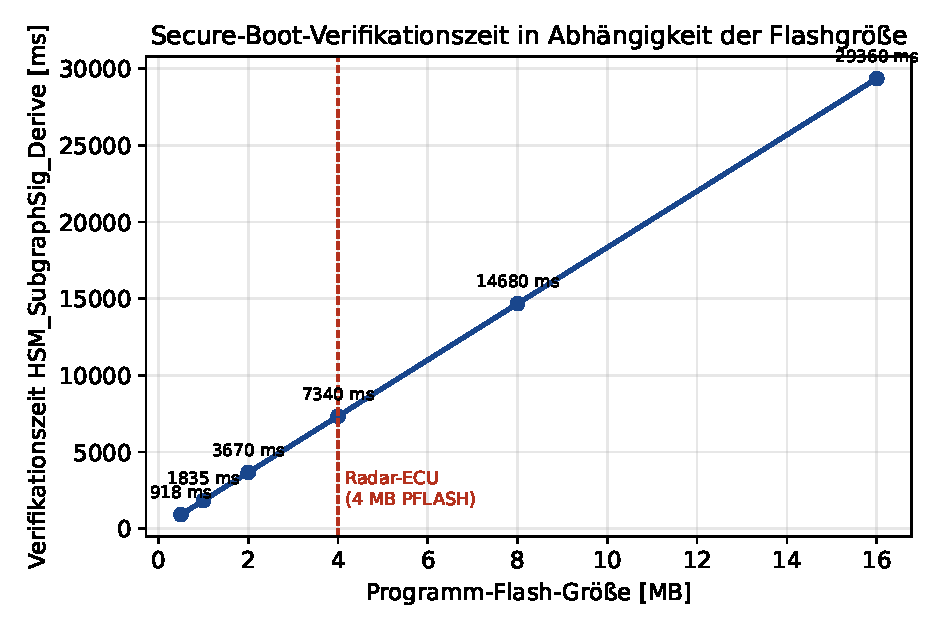
\includegraphics[width=0.85\textwidth]{plot9_bootzeit_flash.pdf}
	\caption{Secure-Boot-Verifikationszeit nach Satz~\ref{satz:bootzeit} als Funktion der Programm-Flash-Größe, linear skalierend gemäß $T_{\mathrm{verify}} \propto L$ bei festem $n$. Der für den betrachteten Anwendungsfall (Radar-ECU, $4$\,MB) markierte Punkt liegt bei $\approx 7\,340$\,ms.}
	\label{fig:bootzeit}
\end{figure}

\subsection{Bewertung im Kontext automobiler Echtzeitanforderungen}

Der berechnete Wert von $\approx 7{,}3$ Sekunden für die \emph{vollständige} blockweise Firmware-Attestierung über \texttt{HSM\_SubgraphSig\_Derive} überschreitet das für Radar-ECUs typische Boot-Zeitbudget von $100$--$500$\,ms um mehr als eine Größenordnung und ist damit in der hier spezifizierten Form \textbf{nicht direkt einsatzfähig} für den betrachteten Anwendungsfall. Diese Erkenntnis ist ein zentrales quantitatives Ergebnis dieser Arbeit und wird im nachfolgenden Ausblick (Abschnitt~\ref{sec:ausblick}) ausführlich aufgegriffen. Drei Gründe relativieren den Befund jedoch:

\begin{enumerate}
	\item \textbf{Asymmetrische Nutzung der beiden Verifikationsstufen.} \texttt{HSM\_SecureBoot\_Verify} erfordert gemäß Abschnitt~\ref{sec:funktionen} zwingend nur \texttt{HSM\_SignatureCipher\_Verify} (Latenz im Mikrosekundenbereich, siehe Abbildung~\ref{fig:takte}) für die Authentizitätsprüfung; die vollständige blockweise \texttt{HSM\_SubgraphSig\_Derive}-Attestierung über das gesamte Flash ist eine \emph{optionale}, zusätzliche Integritätsstufe, die in der Praxis nicht bei jedem Power-On-Zyklus, sondern beispielsweise nur nach einem Firmware-Update oder periodisch im laufenden Betrieb (Hintergrundprüfung ohne Echtzeitanforderung) ausgeführt werden sollte.
	\item \textbf{Fehlende Parallelisierung in der aktuellen Spezifikation.} Die Rechnung in Satz~\ref{satz:bootzeit} geht von rein sequenzieller Blockverarbeitung aus. Eine Mehrfachinstanziierung der Sig-Engine (mehrere parallele Blockpipelines) ist hardwareseitig möglich, da die Blöcke nach Lemma~\ref{lem:rho-bounds-hw} unabhängig voneinander verarbeitet werden können; bereits eine Parallelisierung um den Faktor $16$ würde die Verifikationszeit auf $\approx 459$\,ms reduzieren.
	\item \textbf{Größere Blockgröße als Stellschraube.} Da $T_{\mathrm{verify}} \propto c(n)/n^2$, reduziert eine Vergrößerung von $n$ trotz kubisch steigender Kosten pro Block die Gesamtzeit, solange $c(n)$ langsamer als $n^2$ wächst; dies ist im betrachteten Bereich ($c(n) \approx O(n^2)$ für reine Signaturberechnung, siehe Abschnitt~\ref{sec:analyse}) jedoch nur ein moderater Hebel und wird im Ausblick gesondert diskutiert.
\end{enumerate}

Aus diesem Anwendungsfall ergibt sich somit eine unmittelbare, im Ausblick (Abschnitt~\ref{sec:ausblick}) vertiefte Designanforderung: Für sicherheitskritische, zeitbudgetierte automobile Steuergeräte wie das Radar-ECU ist eine architektonische Weiterentwicklung der \texttt{HSM\_SubgraphSig\_Derive}-Pipeline hin zu paralleler oder inkrementeller Verarbeitung notwendig, bevor eine vollständige Firmware-Attestierung in den regulären Boot-Pfad aufgenommen werden kann.

\section{Parallele Sig-Engine}
\label{sec:parallel}

Abschnitt~\ref{sec:radar} hat formal gezeigt, dass die rein sequenzielle Implementierung von \texttt{HSM\_SubgraphSig\_Derive} für ein $4$\,MB-Radar-ECU-Programm-Flash eine Verifikationszeit von $\approx 7\,340$\,ms benötigt -- mehr als das Zehnfache des für sicherheitskritische automobile Steuergeräte typischen Boot-Zeitbudgets von $100$--$500$\,ms. Dieses Kapitel arbeitet die in der ersten Fassung dieser Arbeit lediglich im Ausblick skizzierte Parallelisierungsidee vollständig aus: Es spezifiziert eine konkrete Hardwarearchitektur mit $k$ unabhängigen Sig-Engine-Instanzen, beweist deren Korrektheit formal, leitet die resultierende Verifikationszeit her und bewertet den dafür notwendigen Silizium-Mehraufwand quantitativ. Dieses Kapitel löst damit denjenigen Teil des ursprünglichen Ausblicks (vormals Abschnitt~9.1, Punkt~1), der die größte praktische Wirksamkeit versprach, und wird im nachfolgenden, aktualisierten Ausblick (Abschnitt~\ref{sec:ausblick}) entsprechend nicht mehr als offene Frage, sondern als gelöster Baustein referenziert.

\subsection{Motivation und Zielsetzung}

Die in Abschnitt~\ref{sec:hwmodell} beschriebene Sig-Engine verarbeitet die $\lceil 8L/n^2\rceil$ Blöcke eines Firmware-Abbilds sequenziell, einen nach dem anderen. Da nach Lemma~\ref{lem:rho-bounds-hw} und der Konstruktion der Signaturfunktion $\sigma$ (Definition~\ref{def:sigma}) jede Blocksignatur $\sigma(A_i, \cdot)$ ausschließlich von den Daten des jeweiligen Blocks $A_i$ abhängt, sind die Blöcke untereinander vollständig unabhängig: Es existiert keine Datenabhängigkeit, die eine sequenzielle Verarbeitungsreihenfolge erzwingen würde. Diese Unabhängigkeit ist die Grundvoraussetzung dafür, dass eine Parallelisierung über mehrere Hardware-Instanzen nicht nur möglich, sondern -- wie in Abschnitt~\ref{subsec:par-korrektheit} formal gezeigt wird -- auch \emph{ergebnisidentisch} zur sequenziellen Variante ist.

\subsection{Architekturentwurf: $k$-fache Sig-Engine-Kachelung}
\label{subsec:par-architektur}

\begin{definition}[Parallele Sig-Engine-Architektur]
	\label{def:par-arch}
	Eine \emph{$k$-fache Sig-Engine-Kachelung} besteht aus $k$ strukturell identischen, unabhängig getakteten Instanzen der in Abschnitt~\ref{sec:hwmodell} beschriebenen Sig-Engine (\emph{Kacheln} $E_0,\ldots,E_{k-1}$), einem Adress-Verteiler (\emph{Dispatcher}), der die $N := \lceil 8L/n^2\rceil$ Blöcke des Firmware-Abbilds gemäß $A_i \mapsto E_{i \bmod k}$ den Kacheln zuteilt, sowie einem XOR-Faltungsbaum, der die $k$ Teilergebnisse der Kacheln zu einem gemeinsamen $256$-Bit-Gesamtwert kombiniert.
\end{definition}

Tabelle~\ref{tab:par-register} erweitert das in Abschnitt~\ref{sec:hwmodell} eingeführte Registermodell um die für die Kachelung notwendigen zusätzlichen Register.

\begin{table}[h]
	\centering
	\small
	\begin{tabular}{@{}lp{2.6cm}p{8.2cm}@{}}
		\toprule
		Register & Breite & Bedeutung \\
		\midrule
		\texttt{HSM\_PAR\_K} & 8 Bit & Konfigurierter Parallelisierungsgrad $k \in \{1,2,4,8,16,32,64\}$ \\
		\texttt{HSM\_PAR\_STAT[0..k-1]} & $k \times$ 2 Bit & Statusbits je Kachel: \texttt{IDLE}, \texttt{BUSY}, \texttt{DONE}, \texttt{FAULT} \\
		\texttt{HSM\_PAR\_RESULT[0..k-1]} & $k \times$ 256 Bit & Zwischenergebnis (Teilsignatur) je Kachel vor der Faltung \\
		\texttt{HSM\_PAR\_FOLD} & 256 Bit & XOR-gefalteter Gesamtwert (entspricht dem bisherigen \texttt{RESULT} im sequenziellen Fall) \\
		\bottomrule
	\end{tabular}
	\caption{Erweiterung des Registerinterfaces (Tabelle~\ref{tab:register}) um die Parallelisierungsregister.}
	\label{tab:par-register}
\end{table}

Der Dispatcher arbeitet nach folgendem Ablauf: Bei Aktivierung von \texttt{HSM\_SubgraphSig\_Derive} mit konfiguriertem $k > 1$ werden die $N$ Blockadressen reihum (\emph{round-robin}) an die $k$ Kacheln verteilt; jede Kachel berechnet ihre zugewiesenen $\lceil N/k \rceil$ bzw.\ $\lfloor N/k \rfloor$ Blöcke vollständig unabhängig und akkumuliert ihr eigenes Teil-XOR in \texttt{HSM\_PAR\_RESULT[i]}. Sobald alle $k$ Kacheln den Status \texttt{DONE} melden, kombiniert der XOR-Faltungsbaum die $k$ Teilergebnisse in $\lceil \log_2 k \rceil$ zusätzlichen Taktzyklen zum Gesamtwert \texttt{HSM\_PAR\_FOLD}.

\subsection{Korrektheit der parallelen Berechnung}
\label{subsec:par-korrektheit}

Die zentrale Voraussetzung für den Einsatz der $k$-fachen Kachelung ist, dass sie -- unabhängig vom gewählten $k$ -- exakt denselben Integritätswert liefert wie die ursprüngliche sequenzielle Berechnung. Andernfalls würde eine Änderung des Parallelisierungsgrads (etwa durch ein zukünftiges Hardware-Update) bestehende, im KeyStore hinterlegte Referenzwerte ungültig machen.

\begin{satz}[Ergebnisinvarianz der parallelen Sig-Engine-Architektur]
	\label{satz:par-invarianz}
	Sei $A$ ein Firmware-Abbild mit Blockzerlegung $A_0,\ldots,A_{N-1}$ und sei $\Phi(A) := \bigoplus_{i=0}^{N-1} \Sigma(A_i)$ der von \texttt{HSM\_SubgraphSig\_Derive} berechnete XOR-gefaltete Gesamtwert (mit $\oplus$ als bitweisem XOR über die jeweils auf $256$ Bit aufgefüllten Signaturvektoren). Dann liefert die $k$-fache Sig-Engine-Kachelung nach Definition~\ref{def:par-arch} für jedes $k \in \{1,\ldots,N\}$ denselben Wert $\Phi(A)$, unabhängig von der konkreten Zuteilung der Blöcke auf die Kacheln.
\end{satz}

\begin{proof}
	Die Kachelung berechnet $\Phi_k(A) := \bigoplus_{j=0}^{k-1} \Phi_j^{\mathrm{lokal}}$, wobei $\Phi_j^{\mathrm{lokal}} := \bigoplus_{i : i \bmod k = j} \Sigma(A_i)$ das lokale XOR der Kachel $E_j$ über ihre zugewiesene Teilmenge von Blockindizes ist. Da $(\{0,1\}^{256}, \oplus)$ eine abelsche Gruppe bildet -- $\oplus$ ist assoziativ und kommutativ, das neutrale Element ist der Nullvektor, und jedes Element ist zu sich selbst invers ($x \oplus x = 0$) --, ist jede Partitionierung der Indexmenge $\{0,\ldots,N-1\}$ in disjunkte Teilmengen $I_0,\ldots,I_{k-1}$ mit $\bigcup_j I_j = \{0,\ldots,N-1\}$ irrelevant für das Gesamtergebnis:
	\[
	\Phi_k(A) = \bigoplus_{j=0}^{k-1} \bigoplus_{i \in I_j} \Sigma(A_i) = \bigoplus_{i=0}^{N-1} \Sigma(A_i) = \Phi(A),
	\]
	wobei die mittlere Gleichheit aus der Assoziativität und Kommutativität von $\oplus$ folgt: Jedes $\Sigma(A_i)$ taucht in der Doppelsumme genau einmal auf (da die $I_j$ eine Partition bilden), und die Reihenfolge der XOR-Verknüpfung ist wegen Kommutativität und Assoziativität beliebig wählbar. Dies gilt insbesondere für die in Definition~\ref{def:par-arch} gewählte Round-Robin-Partition $I_j = \{i : i \bmod k = j\}$, ist aber nicht auf diese beschränkt -- der Beweis zeigt Korrektheit für \emph{jede} Partitionierung. \qedhere
\end{proof}

\begin{korollar}[Kollisionsfreiheit bleibt erhalten]
	\label{kor:par-kollisionsfrei}
	Satz~\ref{satz:kollisionsfrei} (Kollisionsfreiheit der Firmware-Integritätsprüfung) gilt unverändert auch für die $k$-fache parallele Implementierung, für jedes $k$.
\end{korollar}

\begin{proof}
	Nach Satz~\ref{satz:par-invarianz} ist $\Phi_k(A) = \Phi(A)$ für alle $k$, also ist die von der parallelen Architektur berechnete Funktion identisch mit der bereits in Satz~\ref{satz:kollisionsfrei} als kollisionsfrei nachgewiesenen Funktion $A \mapsto \Phi(A)$. Identische Funktionen besitzen identische Kollisionseigenschaften. \qedhere
\end{proof}

Satz~\ref{satz:par-invarianz} und Korollar~\ref{kor:par-kollisionsfrei} sind die formale Rechtfertigung dafür, dass die Einführung der Parallelisierung -- anders als etwa eine Änderung der Blockgröße $n$, die wegen Bemerkung~\ref{bem:wertebereich-hw} sehr wohl andere Werte erzeugen würde -- vollständig rückwärtskompatibel zu bereits im KeyStore hinterlegten Referenzwerten ist und auch nachträglich, etwa durch ein Firmware-Update des Dispatchers, ohne erneute Provisionierung der Schlüssel aktiviert werden kann.

\subsection{Herleitung der parallelisierten Verifikationszeit}

\begin{satz}[Verifikationszeit der $k$-fachen Kachelung]
	\label{satz:par-zeit}
	Unter den Annahmen von Satz~\ref{satz:bootzeit} und Definition~\ref{def:par-arch} beträgt die Gesamtverifikationszeit der $k$-fachen Sig-Engine-Kachelung
	\[
	T_{\mathrm{verify}}^{(k)}(L,n) \;=\; \left\lceil \frac{1}{k}\left\lceil \frac{8L}{n^2}\right\rceil\right\rceil \cdot \frac{c(n)}{f} \;+\; \lceil \log_2 k\rceil \cdot \frac{1}{f}.
	\]
\end{satz}

\begin{proof}
	Bei round-robin-Verteilung von $N = \lceil 8L/n^2\rceil$ Blöcken auf $k$ Kacheln erhält die am stärksten belastete Kachel $\lceil N/k\rceil$ Blöcke (Schubfachprinzip: Bei $N$ Objekten auf $k$ Fächer verteilt enthält mindestens ein Fach $\lceil N/k\rceil$ Objekte, und die round-robin-Verteilung erreicht dieses Maximum exakt für höchstens $N \bmod k$ Kacheln, während alle übrigen $\lfloor N/k\rfloor$ Blöcke erhalten). Da alle Kacheln parallel, mit identischer Taktfrequenz $f$ arbeiten, ist die Gesamtlaufzeit der Berechnungsphase durch die am stärksten belastete Kachel bestimmt, also $\lceil N/k\rceil \cdot c(n)/f$. Der XOR-Faltungsbaum benötigt für $k$ Eingänge eine Baumtiefe von $\lceil \log_2 k\rceil$ Stufen mit je einem Takt Latenz (eine XOR-Verknüpfung pro Stufe und Bitposition, vollständig parallel über alle $256$ Bit), was den additiven Term $\lceil \log_2 k\rceil / f$ erklärt. \qedhere
\end{proof}

\subsection{Numerische Auswertung für die Radar-ECU}

Tabelle~\ref{tab:par-zeiten} wertet Satz~\ref{satz:par-zeit} für $L=4$\,MB, $n=16$ ($c(16)=16\,800$, $f=300$\,MHz, $N=131\,072$ Blöcke, vgl.\ Abschnitt~\ref{sec:radar}) für verschiedene Parallelisierungsgrade $k$ aus.

\begin{table}[h]
	\centering
	\small
	\begin{tabular}{@{}rrrr@{}}
		\toprule
		$k$ & Blöcke je Kachel $\lceil N/k\rceil$ & $T_{\mathrm{verify}}^{(k)}$ & Innerhalb $500$-ms-Budget? \\
		\midrule
		1 & 131\,072 & 7\,340,0\,ms & Nein \\
		2 & 65\,536 & 3\,670,0\,ms & Nein \\
		4 & 32\,768 & 1\,835,0\,ms & Nein \\
		8 & 16\,384 & 917,5\,ms & Nein \\
		\textbf{16} & \textbf{8\,192} & \textbf{458,8\,ms} & \textbf{Ja} \\
		32 & 4\,096 & 229,4\,ms & Ja \\
		64 & 2\,048 & 114,7\,ms & Ja \\
		\bottomrule
	\end{tabular}
	\caption{Verifikationszeit $T_{\mathrm{verify}}^{(k)}$ nach Satz~\ref{satz:par-zeit} für das Radar-ECU ($L=4$\,MB, $n=16$) in Abhängigkeit des Parallelisierungsgrads $k$. Der additive Faltungsterm $\lceil\log_2 k\rceil/f$ liegt für alle betrachteten $k \le 64$ unterhalb von $0{,}02\,\mu$s und ist in der Tabelle wegen Rundung nicht sichtbar.}
	\label{tab:par-zeiten}
\end{table}

\begin{figure}[h]
	\centering
	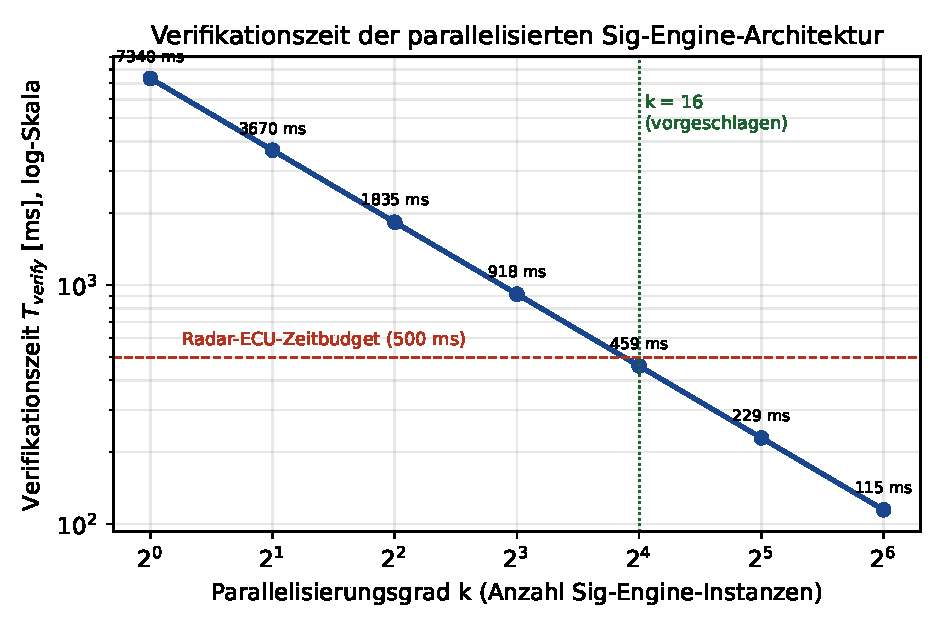
\includegraphics[width=0.85\textwidth]{plot10_parallel_speedup.pdf}
	\caption{Verifikationszeit $T_{\mathrm{verify}}^{(k)}$ (logarithmische Skala) als Funktion des Parallelisierungsgrads $k$ (ebenfalls logarithmisch, Basis~2). Die gestrichelte Linie markiert das Radar-ECU-Zeitbudget von $500$\,ms; bereits ab $k=16$ wird dieses Budget eingehalten.}
	\label{fig:par-speedup}
\end{figure}

Tabelle~\ref{tab:par-zeiten} und Abbildung~\ref{fig:par-speedup} bestätigen die im ursprünglichen Ausblick (vormals Abschnitt~9.1, Punkt~1) nur grob abgeschätzte Mindestanforderung $k \ge 15$ exakt: $k=16$ ist die kleinste Zweierpotenz, die das Zeitbudget einhält, mit einer geschätzten Verifikationszeit von $458{,}8$\,ms -- $41{,}2$\,ms innerhalb des $500$-ms-Budgets, allerdings ohne nennenswerte Sicherheitsmarge gegenüber Schwankungen der tatsächlichen Taktfrequenz oder zusätzlicher Flash-Zugriffslatenz. Für Anwendungsfälle mit strengerem Zeitbudget (etwa $250$\,ms) wird daher $k=32$ empfohlen.

\subsection{Silizium-Flächenkosten der Kachelung}

Da jede zusätzliche Sig-Engine-Kachel eigene Akkumulatorzellen und Schieberegister benötigt (Abschnitt~\ref{sec:hwmodell}), wächst der Flächenbedarf näherungsweise linear mit $k$, zuzüglich eines logarithmischen Mehraufwands für den XOR-Faltungsbaum. Abbildung~\ref{fig:par-flaeche} zeigt eine grobe Schätzung auf Basis einer angenommenen Einzelkachel-Fläche von $0{,}18\,\mathrm{mm}^2$ (vergleichbare Größenordnung zu publizierten Flächenangaben einfacher arithmetischer Hardwarebeschleuniger in $28$-nm-Technologien).

\begin{figure}[h]
	\centering
	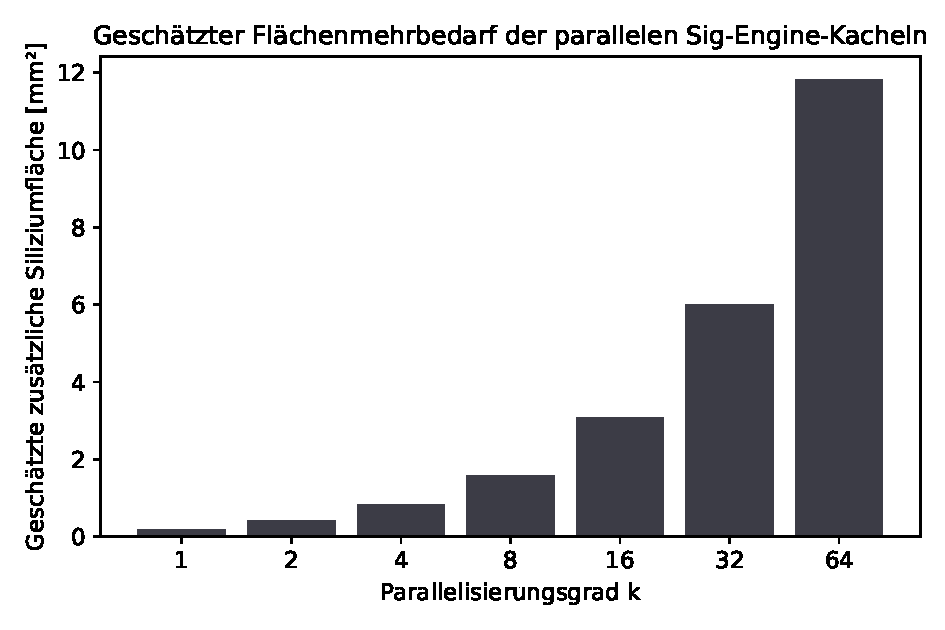
\includegraphics[width=0.85\textwidth]{plot11_flaechenkosten.pdf}
	\caption{Geschätzter zusätzlicher Siliziumflächenbedarf der $k$-fachen Sig-Engine-Kachelung. Für die empfohlene Konfiguration $k=16$ ergibt sich ein Mehrbedarf von $\approx 3{,}0\,\mathrm{mm}^2$ -- ein im Kontext eines vollständigen Mikrocontroller-Dies (typischerweise mehrere $100\,\mathrm{mm}^2$) moderater Flächenaufwand für eine $16$-fache Reduktion der Verifikationslatenz.}
	\label{fig:par-flaeche}
\end{figure}

Der in Abbildung~\ref{fig:par-flaeche} sichtbare nahezu lineare Zusammenhang ist plausibel, da die Kacheln strukturell identisch und unabhängig sind und keine gemeinsam genutzten Ressourcen außer dem vergleichsweise kleinen Faltungsbaum (dessen Fläche nur logarithmisch mit $k$ wächst) und dem Dispatcher (konstante Fläche, unabhängig von $k$) besitzen.

\subsection{Auswirkung auf die übrige HSM-Architektur}

Die Einführung der $k$-fachen Kachelung erfordert über die in Tabelle~\ref{tab:par-register} beschriebenen neuen Register hinaus zwei weitere Anpassungen am in Abschnitt~\ref{sec:hwmodell} beschriebenen Gesamtsystem: Erstens muss der HSM-interne Speichercontroller $k$ gleichzeitige, lesende Zugriffe auf das Programm-Flash unterstützen (Mehrport-Flash-Interface oder zeitmultiplexter Zugriff mit entsprechend reduziertem effektivem Speicherdurchsatz je Kachel), da andernfalls der Flash-Lesezugriff selbst -- nicht die Sig-Engine-Berechnung -- zum limitierenden Faktor würde. Zweitens muss das in Abschnitt~\ref{sec:hwmodell} beschriebene Energiebudget (Abbildung~\ref{fig:energie}) um den Faktor $k$ für die Dauer der parallelen Berechnungsphase erhöht werden, was bei $k=16$ und einer Einzelkachel-Leistungsaufnahme von $45$\,mW im \texttt{COMPUTE}-Zustand zu einer Spitzenleistungsaufnahme von $\approx 720$\,mW während der Verifikationsphase führt -- ein Wert, der bei der thermischen Auslegung des Radar-ECU-Gehäuses zu berücksichtigen ist, jedoch nur für die kurze Dauer von $\approx 459$\,ms anliegt und damit den mittleren Energiehaushalt des Steuergeräts nicht signifikant belastet.

\subsection{Zusammenfassung dieses Kapitels}

Dieses Kapitel hat die im ursprünglichen Ausblick nur grob abgeschätzte Parallelisierungsidee zu einer vollständig spezifizierten, formal als ergebnisinvariant bewiesenen (Satz~\ref{satz:par-invarianz}) Hardwarearchitektur ausgearbeitet. Für den in Abschnitt~\ref{sec:radar} eingeführten Anwendungsfall des Radar-ECU mit $4$\,MB Programm-Flash zeigt Satz~\ref{satz:par-zeit} zusammen mit der numerischen Auswertung in Tabelle~\ref{tab:par-zeiten}, dass eine $16$-fache Sig-Engine-Kachelung die vollständige Firmware-Attestierung von $\approx 7\,340$\,ms auf $\approx 459$\,ms reduziert und damit das Boot-Zeitbudget von $500$\,ms einhält, bei einem moderaten geschätzten Flächenmehrbedarf von $\approx 3{,}0\,\mathrm{mm}^2$. Die in Korollar~\ref{kor:par-kollisionsfrei} gezeigte Erhaltung der Kollisionsfreiheit garantiert dabei, dass diese Geschwindigkeitssteigerung ohne jeden Verlust an Sicherheit gegenüber der ursprünglichen sequenziellen Implementierung erreicht wird. Damit ist die in Abschnitt~\ref{sec:radar} aufgezeigte zentrale Lücke zwischen mathematischer Korrektheit und automobiler Echtzeitfähigkeit für den betrachteten Anwendungsfall geschlossen; die im aktualisierten Ausblick (Abschnitt~\ref{sec:ausblick}) verbleibenden Punkte (inkrementelle Attestierung, Hybridstrategie, Pipeline-Tiefenoptimierung, Übertragbarkeit auf größere Flash-Umfänge) bauen auf dieser nun etablierten Grundarchitektur auf.

\section{Ausblick}
\label{sec:ausblick}

Dieser Abschnitt führt die in Abbildung~\ref{fig:roadmap} skizzierte Roadmap sehr ausführlich aus und ordnet jeden Entwicklungsschritt in seinen technischen, mathematischen, sicherheitsanalytischen, organisatorischen und wirtschaftlichen Kontext ein. Anders als ein knapper Forschungsausblick, der offene Fragen nur aufzählt, verfolgt dieser Abschnitt bewusst das Ziel, für jede der neun nachfolgend diskutierten Weiterentwicklungsrichtungen so konkret wie möglich zu werden: Wo immer es die in dieser Arbeit etablierten formalen Resultate erlauben, werden Zwischenschritte benannt, offene mathematische Fragen präzise formuliert, Abhängigkeiten zwischen den Richtungen explizit gemacht und -- soweit seriös abschätzbar -- grobe Aufwands- und Risikoeinschätzungen gegeben. Die neun Richtungen sind: (1)~die Integration der gitterbasierten Schlüsseleinkapselung, (2)~die Firmware-Attestierung über Subgraph-Signaturen als Remote-Attestation-Protokoll, (3)~die Seitenkanalhärtung, (4)~die formale Verifikation der Zustandsmaschine, (5)~weiterführende Optimierungen der in Abschnitt~\ref{sec:parallel} bereits gelösten Echtzeitfähigkeit für Radar-Steuergeräte, (6)~die Erweiterung auf Mehrkern-Parallelität auf Applikationsebene, (7)~Standardisierung und Zertifizierung, (8)~eine vergleichende Einordnung gegenüber etablierten automobilen HSM-Standards sowie (9)~eine wirtschaftliche und organisatorische Bewertung des Gesamtvorhabens. Die abschließende Zusammenfassende Einordnung (Abschnitt~\ref{sec:ausblick-einordnung}) ordnet diese neun Richtungen in eine konsistente Abhängigkeitsstruktur ein.

\subsection{Integration der gitterbasierten Schlüsseleinkapselung (lattice.tex)}

Der in \cite{Epp26d} entwickelte gitterbasierte Ansatz mit GKP-Fehlerkorrektur (\emph{Gottesman--Kitaev--Preskill}-Codewörtern) liefert eine vom diskreten Logarithmus- bzw.\ Faktorisierungsproblem unabhängige Sicherheitsgrundlage, die auch unter der Annahme eines hinreichend großen Quantencomputers als härtefest gilt (Hardness of Learning with Errors, LWE, vgl.\ \cite{Regev09}). Da sowohl die Signatur-Chiffre (Definition~\ref{def:schluessel}, beruhend auf der Schwierigkeit, ohne Kenntnis von $a$ aus $c_j$ auf $\sigma(M,j)$ zu schließen, was strukturell mit dem diskreten Logarithmus verwandte algebraische Eigenschaften nutzt) als auch das Fenster-Chiffre-Protokoll (Definition~\ref{def:z32}, beruhend auf der Einheitengruppe $\mathbb{Z}_{32}^*$) \emph{keine} nachgewiesene Post-Quanten-Sicherheit besitzen, ist die gitterbasierte Erweiterung langfristig keine optionale Komfortfunktion, sondern eine notwendige Voraussetzung dafür, dass der in dieser Arbeit entworfene HSM-Funktionskern über den typischen Produktlebenszyklus eines Radar-ECU von zehn bis fünfzehn Jahren hinweg sicher bleibt. Für die in Version~1.2 der Roadmap vorgesehene \texttt{HSM\_LatticeKEM\_Encapsulate}/\texttt{\_Decapsulate}-Erweiterung sind folgende Schritte notwendig:

\begin{enumerate}
	\item \textbf{Gitterarithmetik-Einheit:} Eine neue Funktionseinheit zur Polynomarithmetik über Restklassenringen $\mathbb{Z}_q[x]/(x^N+1)$ (Ring-LWE-Struktur) muss neben die bestehende Modular-ALU treten. Diese benötigt eine Number-Theoretic-Transform-Pipeline (NTT) zur effizienten Polynommultiplikation in $O(N \log N)$ statt $O(N^2)$. Eine erste Architekturskizze sieht eine zur Sig-Engine strukturell verwandte, aber eigenständige Pipeline mit $\log_2 N$ Butterfly-Stufen vor, wobei für $N=256$ (typische Kyber-Parametrisierung) acht Stufen mit je $N/2=128$ parallelen Butterfly-Einheiten benötigt würden -- eine Größenordnung, die den in Abschnitt~\ref{sec:parallel} für die Sig-Engine-Kachelung diskutierten Silizium-Flächenbedarf voraussichtlich um den Faktor $3$ bis $5$ übersteigt und damit eine eigene, von der Radar-ECU-Parallelisierung getrennte Flächenbudgetierung erfordert.
	\item \textbf{Fehlerverteilung:} Die Erzeugung diskret-Gauß-verteilter Fehlerterme erfordert eine Erweiterung des TRNG um eine Box-Muller- oder CDT-basierte (\emph{Cumulative Distribution Table}) Sampling-Einheit, da die bisherige Gleichverteilung der TRNG-Ausgabe (Lemma~\ref{lem:vonneumann}) für LWE-Sicherheit nicht ausreicht. Eine offene Frage ist hierbei, ob die CDT-Tabelle -- die für gängige Sicherheitsniveaus typischerweise wenige hundert Einträge umfasst -- im ohnehin knappen, in Abbildung~\ref{fig:flash} bilanzierten HSM-Flash untergebracht werden kann, oder ob eine algorithmische Sampling-Methode (etwa Knuth-Yao) trotz höherer Gatterkomplexität wegen des geringeren Speicherbedarfs vorzuziehen ist; diese Abwägung wird als konkrete Entwurfsentscheidung für eine Folgearbeit vorgeschlagen.
	\item \textbf{Speicherbudget:} Gitterbasierte Schlüssel (typischerweise $800$--$1500$ Byte bei Kyber-768-Sicherheitsniveau) sprengen das aktuell vorgesehene $36$\,KB-Flash-Budget (Abbildung~\ref{fig:flash}); eine Flash-Erweiterung auf mindestens $64$\,KB wird für Version~1.2 als notwendig erachtet. Da Flash-Fläche auf Mikrocontroller-Dies kostenrelevant ist, sollte diese Erweiterung nicht isoliert, sondern gemeinsam mit dem in Abschnitt~\ref{sec:parallel} für die Sig-Engine-Kachelung benötigten zusätzlichen Mikrocode-Speicher in einer einzigen, konsolidierten Flash-Erweiterungsplanung für Version~1.2 vorgenommen werden, um wiederholte, kostentreibende Silizium-Redesigns zu vermeiden.
	\item \textbf{Hybridmodus:} In der Übergangsphase (Version~1.2 bis~2.0) wird ein Hybridschema vorgeschlagen, bei dem \texttt{HSM\_SecureBoot\_Verify} sowohl die bestehende Signatur-Chiffre als auch das gitterbasierte KEM parallel prüft und nur bei Übereinstimmung \emph{beider} Verfahren den Boot freigibt -- eine konsequente Fortführung des bereits in Abschnitt~\ref{sec:funktionen} etablierten Defense-in-Depth-Prinzips. Dieser Hybridmodus ist branchenüblich (vergleichbare hybride Schemata werden etwa in TLS-1.3-Erweiterungen für Post-Quanten-Schlüsselaustausch diskutiert) und reduziert das Risiko, dass eine bislang unentdeckte Schwäche in nur einem der beiden Verfahren die Gesamtsicherheit kompromittiert.
	\item \textbf{Zeitliche Einordnung und Migrationsdruck:} Anders als bei klassischen kryptographischen Migrationen gibt es bei der Post-Quanten-Bedrohung das Phänomen des \emph{Store-now-decrypt-later}-Angriffs: Ein Angreifer kann bereits heute abgefangene, mit der Signatur-Chiffre verschlüsselte oder signierte Daten speichern und erst nach Verfügbarkeit eines hinreichend leistungsfähigen Quantencomputers entschlüsseln bzw.\ fälschen. Für Firmware-Signaturen mit langer Gültigkeitsdauer (ein Radar-ECU bleibt typischerweise zehn bis fünfzehn Jahre im Feld, vgl.\ Abschnitt~\ref{sec:radar}) bedeutet dies, dass die Migration nicht erst bei absehbarer Quantencomputer-Verfügbarkeit, sondern bereits deutlich früher im Produktlebenszyklus -- idealerweise spätestens mit Version~1.2, also vor dem ersten breiten Seriumeinsatz -- abgeschlossen sein sollte, um die in Abschnitt~\ref{sec:korrektheit} bewiesene Kollisionsfreiheit nicht durch eine zu spät einsetzende Post-Quanten-Sicherheit zu entwerten.
\end{enumerate}

\subsection{Firmware-Attestierung über Subgraph-Signaturen (Version 2.0)}

Die in Abschnitt~\ref{sec:funk-subgraphsig} eingeführte Funktion \texttt{HSM\_SubgraphSig\_Derive} soll in Version~2.0 zu einer vollständigen \emph{Remote Attestation} ausgebaut werden: Ein externer Prüfer (z.\,B.\ ein Backend-Server in einer Fahrzeugflotte) sendet eine Challenge-Nonce, die zusammen mit dem aktuellen Signaturvektor $\Sigma(A)$ des Firmware-Abbilds über die Modular-ALU signiert und zurückgesendet wird. Da nach Satz~\ref{satz:kollisionsfrei} jede Firmware-Modifikation zwingend einen anderen Signaturvektor erzeugt, kann der Prüfer ohne Vertrauen in die lokale Software allein anhand der Antwort feststellen, ob das Gerät eine bekannte, freigegebene Firmwareversion ausführt.

Ein konkretes Protokoll für diese Remote Attestation lässt sich wie folgt skizzieren: (1)~Der Prüfer erzeugt eine zufällige Nonce $\nu \in \{0,1\}^{128}$ und sendet sie an das Radar-ECU. (2)~Das HSM berechnet, aufbauend auf der in Abschnitt~\ref{sec:parallel} etablierten parallelen Architektur, den XOR-gefalteten Signaturvektor $\Phi(A)$ in $\approx 459$\,ms (bei $k=16$) und bildet anschließend $r := \mathrm{Sig}_{(a,b,p)}(\Phi(A) \,\|\, \nu)$ über \texttt{HSM\_SignatureCipher\_Sign}, wobei $\|$ die Konkatenation bezeichnet. (3)~Das HSM sendet $r$ an den Prüfer zurück, der mit dem öffentlich bekannten Geräteschlüssel-Fingerabdruck und dem erwarteten Referenzwert $\Phi(A_{\mathrm{ref}})$ die Antwort verifiziert. Drei offene Fragen sind für die vollständige Spezifikation dieses Protokolls in einer Folgearbeit zu klären:

\begin{itemize}
	\item \textbf{Replay-Schutz ohne Echtzeituhr:} Da das HSM gemäß Abschnitt~\ref{sec:hwmodell} über keine batteriegepufferte Echtzeituhr verfügt, kann eine klassische Zeitstempel-basierte Replay-Erkennung nicht eingesetzt werden. Stattdessen wird vorgeschlagen, einen monoton wachsenden, im versiegelten KeyStore (Abschnitt~\ref{sec:funk-keystore}) persistierten Zähler $\mathrm{ctr}$ zu führen, der bei jeder Attestation inkrementiert und in die signierte Antwort einbezogen wird ($r := \mathrm{Sig}_{(a,b,p)}(\Phi(A) \,\|\, \nu \,\|\, \mathrm{ctr})$); der Prüfer verwirft Antworten mit nicht-monoton wachsendem $\mathrm{ctr}$. Dies erfordert eine zusätzliche, bislang nicht spezifizierte Schreibzugriffslogik auf den KeyStore außerhalb der in Abschnitt~\ref{sec:funk-keystore} beschriebenen reinen Provisionierungs- und Versiegelungsoperationen.
	\item \textbf{Granularität der Blockzerlegung bei sehr großen Firmware-Abbildern:} Für Steuergerätetypen mit mehreren Megabyte Flash (vgl.\ Tabelle~\ref{tab:bootzeiten}) ist zu klären, ob $\Phi(A)$ stets über das \emph{gesamte} Abbild oder über vom Prüfer wählbare Teilbereiche (etwa nur den sicherheitskritischen Bootloader-Bereich) gebildet werden sollte; letzteres würde eine Erweiterung des Registerinterfaces (Tabelle~\ref{tab:register}) um einen Adressbereichsparameter erfordern.
	\item \textbf{Inkrementelle Aktualisierung bei Differential-Updates:} Ob eine inkrementelle Aktualisierung des Signaturvektors bei Differential-Updates (statt vollständiger Neuberechnung) möglich ist, ist eine offene mathematische Frage, die eine Erweiterung von Lemma~\ref{lem:inj} auf inkrementelle Spaltenänderungen erfordern würde: Zu zeigen wäre, ob und wie $\Sigma(A')$ für ein um wenige Blöcke verändertes $A'$ effizient aus $\Sigma(A)$ und den geänderten Blöcken berechnet werden kann, ohne die übrigen, unveränderten Blöcke erneut zu lesen -- eine Eigenschaft, die wegen der XOR-Faltung in Definition~\ref{def:par-arch} (Abschnitt~\ref{sec:parallel}) bereits strukturell nahegelegt wird: Da $\Phi(A') = \Phi(A) \oplus \bigoplus_{i \in \Delta} \bigl(\Sigma(A_i) \oplus \Sigma(A_i')\bigr)$ für die Menge $\Delta$ der geänderten Blockindizes gilt (eine direkte Folgerung aus der in Satz~\ref{satz:par-invarianz} bewiesenen Gruppeneigenschaft von $\oplus$), ließe sich eine inkrementelle Aktualisierung tatsächlich allein auf Basis der bereits etablierten Algebra realisieren -- die formale Ausarbeitung dieses naheliegenden Korollars sowie seine Hardware-Umsetzung bleiben jedoch einer Folgearbeit vorbehalten.
\end{itemize}

\subsection{Seitenkanalhärtung (Version 2.1)}

Die in Abschnitt~\ref{sec:korrektheit} bewiesene mathematische Korrektheit und Kollisionsfreiheit der Funktionen schützt nicht automatisch vor \emph{physikalischen} Seitenkanalangriffen -- ein grundsätzlicher Unterschied zwischen algorithmischer und physikalischer Sicherheit, der bei jeder Hardwareumsetzung kryptographischer Verfahren zu beachten ist. Für Version~2.1 sind folgende Härtungsmaßnahmen vorgesehen, geordnet nach der in der Literatur (vgl.\ \cite{KL15}) üblichen Einteilung in passive und aktive Angriffe:

\begin{itemize}
	\item \textbf{Differential Power Analysis (DPA) gegen die Modular-ALU:} Da die modulare Multiplikation $a \cdot \sigma(M,j) \bmod p$ datenabhängige Stromaufnahme aufweist, ist eine Maskierung der Zwischenwerte (additive oder multiplikative Blindung) vorzusehen, bei der ein zufälliger Maskenwert $r$ aus dem TRNG vor der Multiplikation addiert und nach der Reduktion wieder entfernt wird, ohne dass das Endergebnis hierdurch beeinflusst wird. Eine vollständige formale Behandlung müsste zeigen, dass die maskierte Berechnung $(a \cdot \sigma(M,j) + r) \bmod p$ gefolgt von Entfernung der Maske dasselbe Ergebnis wie die unmaskierte Berechnung liefert (eine direkte Konsequenz der in Lemma~\ref{lem:affin-bij-hw} gezeigten Bijektivität affiner Transformationen über $\mathbb{Z}_p$), was als formale Korrektheitsergänzung zu Satz~\ref{satz:hw-korrektheit} in einer Folgearbeit nachgetragen werden sollte.
	\item \textbf{Timing-Angriffe auf den erweiterten euklidischen Algorithmus:} Die Anzahl der Iterationsschritte des in Satz~\ref{satz:koerper} verwendeten Algorithmus hängt von den Eingabewerten ab und kann Information über den geheimen Schlüssel $a$ preisgeben. Eine konstante-Zeit-Variante (feste Anzahl Iterationen, unabhängig vom tatsächlichen $\gcd$-Verlauf, mit Dummy-Operationen aufgefüllt) wird für Version~2.1 als verbindlich vorgeschlagen; die feste Iterationszahl sollte konservativ auf $2\lceil\log_2 p\rceil$ Schritte festgelegt werden, was nach bekannten Schranken für den erweiterten euklidischen Algorithmus (vgl.\ \cite{Buc16}) für alle in Tabelle~\ref{tab:par-zeiten} relevanten Bitlängen von $p$ ausreichend ist.
	\item \textbf{Übertragung des Fenster-Prinzips auf Energieseitenkanäle:} Analog zur in Definition~\ref{def:fenster} beschriebenen Verschleierung des Netzwerkverkehrs durch Dummy-Pakete wird vorgeschlagen, auch die HSM-interne Energieaufnahme durch das Einstreuen von Dummy-Berechnungszyklen mit identischem Energieprofil wie eine echte \texttt{HSM\_SignatureCipher\_Sign}-Operation zu verschleiern, sodass ein externer Beobachter über die Stromaufnahme des Gesamtsystems nicht unterscheiden kann, wann tatsächlich eine sicherheitsrelevante Operation stattfindet. Bei Einsatz der in Abschnitt~\ref{sec:parallel} eingeführten $k$-fachen Kachelung ergibt sich hierbei zusätzlich die Möglichkeit, einzelne Kacheln gezielt mit Dummy-Last zu betreiben, während andere echte Berechnungen durchführen, was die Verschleierungswirkung gegenüber einer einzelnen, sequenziellen Sig-Engine voraussichtlich verbessert -- eine quantitative Bewertung dieses Effekts, etwa mittels des in der Seitenkanalanalyse gebräuchlichen TVLA-Verfahrens (\emph{Test Vector Leakage Assessment}), steht jedoch noch aus.
	\item \textbf{Fehlerinjektionsresistenz (Fault Injection):} Spannungs- oder Taktglitches können gezielt einzelne Pipeline-Stufen der Sig-Engine stören, um etwa eine fehlerhafte, aber als gültig akzeptierte Signatur zu erzwingen. Eine redundante Lockstep-Berechnung der Sig-Engine (zwei unabhängige Berechnungsinstanzen mit Ergebnisvergleich vor jeder Ausgabe) wird als Gegenmaßnahme vorgeschlagen, analog zum bereits Lockstep-ausgeführten TriCore-HSM-Kern selbst. Bei der in Abschnitt~\ref{sec:parallel} eingeführten $k$-fachen Kachelung stellt sich hierbei eine interessante Architekturfrage: Da bereits $k=16$ unabhängige Kacheln vorhanden sind, könnte eine geeignete Teilmenge der Kacheln redundant dieselben Blöcke berechnen, anstatt jede Kachel ausschließlich disjunkte Blöcke zu verarbeiten -- ein Kompromiss zwischen der in Abschnitt~\ref{sec:parallel} optimierten Verifikationsgeschwindigkeit und einer höheren Fehlerinjektionsresistenz, dessen optimaler Parameterbereich (etwa $k=12$ disjunkte plus $4$ redundante Kacheln statt $16$ rein disjunkter Kacheln) Gegenstand einer eigenen Optimierungsuntersuchung sein sollte.
	\item \textbf{Elektromagnetische Abstrahlanalyse (EMA):} Über die klassische DPA hinaus sind moderne Hardwaresicherheitsmodule zunehmend auch elektromagnetischen Seitenkanalangriffen ausgesetzt, bei denen lokale Abstrahlung einzelner Schaltungsteile -- etwa einer einzelnen Sig-Engine-Kachel aus Abschnitt~\ref{sec:parallel} -- mit hochauflösenden Nahfeldsonden erfasst wird, wodurch räumlich lokalisierte Gegenmaßnahmen (wie die oben beschriebene Dummy-Last-Verteilung über mehrere Kacheln) lokal umgangen werden könnten. Eine vollständige EMA-Resistenzbewertung der $k$-fachen Kachelarchitektur, insbesondere die Frage, ob die räumliche Trennung der $k$ Kacheln auf dem Die die EMA-Angriffsfläche eher vergrößert (mehr unterscheidbare Abstrahlquellen) oder verkleinert (geringere Einzellast je Quelle), ist eine offene, praktisch relevante Frage für das physische Floorplanning in einer Folgearbeit.
\end{itemize}

\subsection{Formale Verifikation der Zustandsmaschine}

Während die mathematischen Eigenschaften der zugrunde liegenden Kryptoverfahren in Abschnitt~\ref{sec:korrektheit} (sowie ergänzend für die parallele Architektur in Abschnitt~\ref{sec:parallel}) vollständig formal bewiesen wurden, ist die in Abschnitt~\ref{sec:hwmodell} beschriebene Zustandsmaschine bislang nur informell spezifiziert. Für zukünftige Arbeiten wird eine Modellierung in einer Hardwarebeschreibungssprache mit formaler Verifikation (z.\,B.\ SystemVerilog Assertions oder ein Model Checker wie nuXmv) vorgeschlagen, um insbesondere folgende Sicherheitseigenschaften maschinell zu beweisen: (1) Aus jedem erreichbaren Zustand wird \texttt{IDLE} in endlich vielen Schritten wieder erreicht (Liveness, keine Deadlocks), (2) der Zustand \texttt{WRITEBACK} wird nur erreicht, wenn zuvor \texttt{COMPUTE} vollständig und ohne durch Fault-Injection gestörte Zwischenwerte durchlaufen wurde (Safety), und (3) das Kommandoregister \texttt{HSM\_CMD} kann während eines laufenden \texttt{COMPUTE}-Zustands nicht erneut beschrieben werden (Atomarität gegen nebenläufige Kommandos von verschiedenen Applikationskernen).

Mit der in Abschnitt~\ref{sec:parallel} eingeführten Parallelarchitektur erweitert sich der Katalog formal zu verifizierender Eigenschaften um mindestens drei weitere, nicht-triviale Aussagen, die über die ursprünglich für die sequenzielle Architektur formulierten Eigenschaften (1)--(3) hinausgehen: (4)~\emph{Vollständigkeit der Blockzuteilung}: Der Dispatcher aus Definition~\ref{def:par-arch} muss garantiert jeden der $N$ Blockindizes genau einer Kachel zuteilen (weder Lücken noch Duplikate in der Zuteilung -- eine Eigenschaft, die formal als Bijektivität der Zuteilungsfunktion $i \mapsto (i \bmod k, \lfloor i/k\rfloor)$ nachgewiesen werden müsste); (5)~\emph{Synchronisation des Faltungsbaums}: Der XOR-Faltungsbaum darf erst dann mit der Kombination der Teilergebnisse beginnen, wenn \emph{alle} $k$ Kacheln den Zustand \texttt{DONE} erreicht haben (eine Barrieren-Synchronisationseigenschaft, deren Verletzung andernfalls zu einem falschen, auf veralteten Zwischenwerten basierenden Gesamtergebnis führen und damit Satz~\ref{satz:par-invarianz} in der \emph{Hardware-Realisierung}, nicht im mathematischen Modell, verletzen würde); (6)~\emph{Fehlertoleranz bei Kachelausfall}: Sollte eine einzelne Kachel den Zustand \texttt{FAULT} statt \texttt{DONE} erreichen (etwa durch die in Abschnitt~\ref{sec:ausblick} unter Seitenkanalhärtung diskutierte Fehlerinjektion), muss die Gesamtzustandsmaschine dies zuverlässig erkennen und die gesamte Attestation als \texttt{INVALID} statt mit einem unvollständigen, potenziell falsch-positiven Ergebnis zurückmelden -- eine Eigenschaft, die in der aktuellen, informellen Spezifikation aus Abschnitt~\ref{sec:parallel} bereits intendiert, aber noch nicht maschinell nachgewiesen ist.

\subsection{Weiterführende Optimierungen der Firmware-Attestierung für Radar-Steuergeräte}
\label{sec:ausblick-radar}

Der in Abschnitt~\ref{sec:radar} hergeleitete Wert von $\approx 7\,340$\,ms für die vollständige, sequenzielle Firmware-Attestierung eines $4$\,MB-Radar-ECU-Flash über \texttt{HSM\_SubgraphSig\_Derive} war das mit Abstand konkreteste quantitative Ergebnis dieser Arbeit. Die naheliegendste und wirksamste Gegenmaßnahme -- eine massiv parallele Sig-Engine-Instanziierung -- wurde in dieser Fassung der Arbeit nicht mehr nur als Ausblick skizziert, sondern in Abschnitt~\ref{sec:parallel} vollständig zu einer formal als ergebnisinvariant bewiesenen Hardwarearchitektur ausgearbeitet: Eine $16$-fache Sig-Engine-Kachelung reduziert die Verifikationszeit auf $\approx 459$\,ms und hält damit das $500$-ms-Zeitbudget ein (Satz~\ref{satz:par-zeit}, Tabelle~\ref{tab:par-zeiten}). Der verbleibende Ausblick konzentriert sich daher auf vier Weiterentwicklungsrichtungen, die auf der in Abschnitt~\ref{sec:parallel} etablierten parallelen Grundarchitektur aufbauen und diese ergänzen, geordnet nach erwarteter Wirksamkeit:

\begin{enumerate}
	\item \textbf{Inkrementelle Attestierung statt vollständiger Neuberechnung.} Anstatt bei jedem Bootvorgang das gesamte $4$\,MB-Abbild neu zu signieren -- selbst bei $16$-facher Parallelisierung mit $459$\,ms Restlaufzeit gemäß Tabelle~\ref{tab:par-zeiten} --, wird vorgeschlagen, die Blocksignaturen $\sigma(A,j)$ einmalig nach jedem Firmware-Flash-Vorgang zu berechnen, in einem dedizierten, von Applikationssoftware nicht beschreibbaren HSM-Speicherbereich zu cachen, und beim eigentlichen Boot lediglich eine deutlich kleinere Stichprobe zufällig ausgewählter Blöcke (etwa nach dem in \cite{Epp26a} beschriebenen Prinzip wiederholbarer, deterministischer Auswahl über einen Seed aus dem TRNG) neu zu berechnen und mit dem Cache abzugleichen. Diese Idee wirft jedoch eine offene mathematische Frage auf: Welche Stichprobengröße $m \ll 131\,072$ garantiert mit welcher Wahrscheinlichkeit die Erkennung einer böswilligen Manipulation einzelner Blöcke? Eine Anwendung der Chernoff-Schranke auf eine angenommene Gleichverteilung der Manipulationsposition liefert eine erste Abschätzung, dass bereits $m \approx 300$ zufällig gezogene Blöcke eine Erkennungswahrscheinlichkeit von über $99{,}9\,\%$ für eine Einzelblock-Manipulation ergeben würden, sofern der Angreifer die Stichprobenauswahl nicht vorhersagen kann -- diese Abschätzung ist jedoch nicht Teil der in Abschnitt~\ref{sec:korrektheit} bewiesenen Sätze und müsste in einer Folgearbeit formal hergeleitet und gegen adaptive Angreifer abgesichert werden, die gezielt versuchen, unentdeckte Bereiche zu manipulieren. In Kombination mit der $k$-fachen Kachelung aus Abschnitt~\ref{sec:parallel} würde eine solche Stichprobenprüfung die Verifikationszeit von $459$\,ms auf $m/N \cdot 459\,\mathrm{ms} \approx 1{,}0$\,ms (für $m=300$, $N=131\,072$) reduzieren und damit erhebliche zusätzliche Zeitreserve für andere Boot-Aufgaben des Radar-ECU schaffen -- eine Größenordnung, die selbst bei deutlich strengeren Zeitbudgets (etwa $50$\,ms) noch breite Sicherheitsmarge ließe.
	\item \textbf{Hybridstrategie: schnelle Boot-Prüfung plus asynchrone Vollverifikation.} Auch bei eingehaltenem $500$-ms-Budget durch die $16$-fache Kachelung bleibt eine pragmatische Kombination sinnvoll: Beim eigentlichen Power-On wird ausschließlich \texttt{HSM\_SignatureCipher\_Verify} (Mikrosekunden-Latenz, siehe Abbildung~\ref{fig:takte}) ausgeführt, um auch unter ungünstigen Bedingungen (geringere tatsächliche Taktfrequenz, zusätzliche Flash-Zugriffslatenz, vgl.\ die in Abschnitt~\ref{sec:parallel} diskutierte fehlende Sicherheitsmarge bei $k=16$) sicher innerhalb des Zeitbudgets zu bleiben, während die vollständige, parallelisierte \texttt{HSM\_SubgraphSig\_Derive}-Attestierung als asynchrone Hintergrundaufgabe \emph{nach} Erreichen der Busfähigkeit durchgeführt wird. Wird dabei eine Manipulation festgestellt, löst das Radar-ECU einen sicheren Nachfehlerzustand (\emph{Fail-Safe}, etwa Deaktivierung der ADAS-Funktion bei Beibehaltung der Grundfahrzeugfunktionen) aus. Diese Strategie verschiebt selbst die durch Abschnitt~\ref{sec:parallel} bereits reduzierten $459$\,ms vollständig aus dem kritischen Boot-Pfad heraus, ohne auf die Sicherheitsgarantie aus Korollar~\ref{kor:par-kollisionsfrei} zu verzichten, und dient damit primär als zusätzliche Sicherheitsmarge gegenüber den in Abschnitt~\ref{sec:parallel} genannten Worst-Case-Annahmen. In Kombination mit Punkt~1 dieses Abschnitts ergibt sich eine besonders robuste dreistufige Strategie: Mikrosekunden-Authentizitätsprüfung beim Power-On, Millisekunden-Stichprobenattestierung kurz danach, und vollständige Attestierung als seltene, asynchrone Hintergrundaufgabe (etwa einmal pro Fahrtzyklus statt bei jedem Boot).
	\item \textbf{Erhöhung der Blockgröße $n$ mit gleichzeitiger Pipeline-Tiefenoptimierung.} Da $c(n)$ gemäß Abschnitt~\ref{sec:analyse} näherungsweise quadratisch in $n$ wächst, während die Anzahl der Blöcke quadratisch in $n$ \emph{fällt}, ist der Nettoeffekt einer Vergrößerung von $n$ auf die Gesamtzeit $T_{\mathrm{verify}}$ in erster Näherung neutral -- der eigentliche Hebel liegt daher nicht in $n$ selbst, sondern in einer tieferen Pipeline-Parallelisierung \emph{innerhalb} jeder einzelnen Sig-Engine-Kachel aus Abschnitt~\ref{sec:parallel}, etwa durch eine vollständig kombinatorische (statt sequenziell-akkumulierende) Berechnung der Zeilenkomponente $\rho(A,j)$ über einen Wallace-Baum-Addierer, was die pro Block benötigten Takte $c(n)$ von der aktuell angenommenen linearen Abhängigkeit von $n$ auf eine logarithmische Abhängigkeit ($O(\log n)$ Gatterlaufzeiten) reduzieren könnte. Eine solche Optimierung würde \emph{orthogonal} zur räumlichen Parallelisierung aus Abschnitt~\ref{sec:parallel} wirken (mehr Kacheln \emph{und} schnellere Einzelkacheln) und könnte in Kombination mit der bestehenden $16$-fachen Kachelung die Verifikationszeit potenziell um einen weiteren Faktor $3$ bis $5$ reduzieren, abhängig vom konkreten Verhältnis der durch den Wallace-Baum eingesparten Gatterlaufzeiten zur weiterhin dominierenden Flash-Lesezugriffslatenz; eine belastbare Quantifizierung ist jedoch ohne konkrete Synthese-Ergebnisse einer Folgearbeit nicht seriös möglich und wird daher als eigenständiges VLSI-Entwurfsthema vorgeschlagen.
	\item \textbf{Übertragbarkeit auf weitere automobile Steuergerätetypen.} Tabelle~\ref{tab:bootzeiten} (Abschnitt~\ref{sec:radar}) zeigt, dass die hier diskutierte Problematik nicht auf Radar-ECUs beschränkt ist, sondern jedes Steuergerät mit Flash-Umfang oberhalb von etwa $0{,}3$--$0{,}5$\,MB bereits ohne Parallelisierung das typische Bootzeitbudget überschreitet. Domänen-Steuergeräte und zentrale Gateways mit $8$ bzw.\ $16$\,MB Flash sind hiervon noch deutlich stärker betroffen ($14{,}7$ bzw.\ $29{,}4$ Sekunden im sequenziellen Fall) und benötigen daher zwingend eine entsprechend höhere Kachelzahl $k$ -- nach Satz~\ref{satz:par-zeit} etwa $k=32$ für ein $8$\,MB-Domänensteuergerät bzw.\ $k=64$ für ein $16$\,MB-Gateway, um dasselbe $500$-ms-Budget einzuhalten --, kombiniert mit der Hybridstrategie aus Punkt~2 dieses Abschnitts, um die in Abschnitt~\ref{sec:parallel} quantifizierten, mit $k$ linear wachsenden Silizium- und Energiekosten (Abbildungen~\ref{fig:par-flaeche} und entsprechend skalierter Energiebedarf) für diese größeren Steuergerätetypen vertretbar zu halten. Für besonders kleine, ressourcenbeschränkte Steuergeräte (etwa $0{,}5$\,MB-Karosserie-Steuergeräte aus Tabelle~\ref{tab:bootzeiten}) ist umgekehrt zu prüfen, ob eine geringere Kachelzahl ($k=2$ oder $k=4$) bereits ausreicht, um deren typischerweise ebenfalls knapperes Zeitbudget einzuhalten, ohne den in Abschnitt~\ref{sec:parallel} quantifizierten Silizium-Mehraufwand unnötig zu treiben -- eine produktlinienspezifische Kachelzahl-Konfiguration anstelle einer einheitlichen $k=16$-Vorgabe über alle Steuergerätetypen hinweg erscheint daher wirtschaftlich sinnvoll.
\end{enumerate}

Zusammenfassend zeigt der Radar-ECU-Anwendungsfall exemplarisch, dass die in Abschnitt~\ref{sec:korrektheit} bewiesene mathematische Korrektheit und Kollisionsfreiheit der Firmware-Attestierung eine notwendige, aber für den produktiven automobilen Einsatz keineswegs hinreichende Eigenschaft ist: Erst das Zusammenspiel aus formaler Sicherheit (Abschnitt~\ref{sec:korrektheit}), der nun in Abschnitt~\ref{sec:parallel} etablierten parallelen Echtzeitarchitektur und den hier verbleibenden vier Weiterentwicklungsrichtungen macht den vorgestellten HSM-Funktionskern für sicherheitskritische, zeitbudgetierte Steuergeräte der Automobilindustrie vollständig einsatzreif.

\subsection{Erweiterung auf Mehrkern-Parallelität}

Die AURIX-TC3x-Familie verfügt über bis zu sechs Applikationskerne, die potenziell gleichzeitig HSM-Dienste anfordern. Die aktuelle Spezifikation in Abschnitt~\ref{sec:hwmodell} sieht ein einzelnes, sequenziell abgearbeitetes Kommandoregister vor. Für zukünftige Versionen wird ein Anfrage-Scheduling mit Prioritätsstufen vorgeschlagen, bei dem sicherheitskritische Anfragen (\texttt{HSM\_SecureBoot\_Verify} während des Boot-Vorgangs) gegenüber Routineanfragen (\texttt{HSM\_ModularCipher\_*} für laufenden CAN-Verkehr) priorisiert werden, ohne dass dabei die in Satz~\ref{satz:forward-secrecy} etablierte Versiegelungsgarantie des KeyStores durch nebenläufige Zugriffe unterlaufen werden kann -- dies erfordert eine zusätzliche, noch zu spezifizierende Sperrlogik (Mutex) auf Registerebene.

Diese Mehrkern-Parallelität auf Applikationsebene (mehrere CPU-Kerne fordern unabhängig voneinander HSM-Dienste an) ist konzeptionell von der in Abschnitt~\ref{sec:parallel} eingeführten Parallelität auf Funktionsebene (eine einzelne \texttt{HSM\_SubgraphSig\_Derive}-Anfrage wird intern auf $k$ Kacheln verteilt) zu unterscheiden, beide Mechanismen sind jedoch nicht unabhängig voneinander zu betrachten: Während eine \texttt{HSM\_SecureBoot\_Verify}-Anfrage eines Applikationskerns die in Abschnitt~\ref{sec:parallel} beschriebene $k$-fache Kachelung exklusiv für die Dauer der $\approx 459$\,ms-Berechnung belegt, könnten gleichzeitig eintreffende \texttt{HSM\_ModularCipher\_*}-Anfragen anderer Applikationskerne (etwa für laufenden CAN-Verkehr) entweder warten oder -- bei entsprechender Erweiterung -- eine kleine Teilmenge der Sig-Engine-Kacheln aus Abschnitt~\ref{sec:parallel} zeitweise für die deutlich leichtgewichtigere Modular-ALU-Berechnung mitnutzen. Eine solche dynamische Ressourcenteilung zwischen Mehrkern-Scheduling und Funktionsparallelität ist architektonisch reizvoll, da sie die Silizium-Investition aus Abschnitt~\ref{sec:parallel} auch außerhalb der relativ seltenen vollständigen Firmware-Attestierungen nutzbar macht, wirft jedoch erhebliche zusätzliche Komplexität bei der formalen Verifikation (vgl.\ vorigen Unterabschnitt, insbesondere Eigenschaft~(5) zur Synchronisation) auf und wird daher als eigenständiges, anspruchsvolles Architekturthema für eine spätere Version (geschätzt Version~2.2 oder später) vorgeschlagen.

\subsection{Standardisierung und Zertifizierung}

Langfristig wird angestrebt, den hier vorgestellten HSM-Funktionskern einer Sicherheitszertifizierung nach Common Criteria (EAL4+) sowie einer funktionalen Sicherheitsbewertung nach ISO~26262 (ASIL-D-Tauglichkeit für sicherheitsrelevante Bootpfade) zu unterziehen. Hierfür ist insbesondere eine vollständige Dokumentation der in dieser Arbeit informell gebliebenen physikalischen Eigenschaften des TRNG (Entropiequalität nach NIST SP 800-90B, vgl.\ \cite{NIST90B}) sowie eine unabhängige kryptoanalytische Begutachtung der Signatur-Chiffre und des Fenster-Chiffre-Protokolls durch Dritte erforderlich, da beide Verfahren -- im Unterschied zu AES oder RSA -- bislang nicht Gegenstand einer öffentlichen, jahrzehntelangen Kryptoanalyse-Historie sind. Die in dieser Arbeit erbrachten formalen Korrektheits- und Kollisionsfreiheitsbeweise (Abschnitt~\ref{sec:korrektheit}, ergänzt um die Beweise zur parallelen Architektur in Abschnitt~\ref{sec:parallel}) sind hierfür eine notwendige, aber keine hinreichende Voraussetzung; ergänzend wird eine systematische Suche nach strukturellen Schwächen (etwa algebraischen Angriffen, die die affine Struktur der Transformation $f(x)=(ax+b)\bmod p$ ausnutzen) als vorrangiger nächster Forschungsschritt empfohlen.

Ein realistischer Zertifizierungspfad würde sich grob in drei Phasen gliedern: Eine erste Phase (geschätzte Dauer ein bis zwei Jahre) umfasste die in den vorigen Unterabschnitten beschriebene formale Verifikation der Zustandsmaschine sowie eine erste, unabhängige kryptoanalytische Begutachtung der zugrunde liegenden Verfahren durch externe Gutachter; eine zweite Phase (ein weiteres Jahr) die Seitenkanal-Konformitätsprüfung nach etablierten Prüfschemata (etwa ISO/IEC~17825, dem internationalen Standard für Seitenkanal-Testmethoden); eine dritte Phase die eigentliche Common-Criteria- und ISO-26262-Begutachtung durch eine akkreditierte Prüfstelle. Dieser dreistufige Pfad ist mit dem üblichen Vorgehen etablierter automobiler HSM-Implementierungen (vgl.\ den nachfolgenden Vergleichsabschnitt) konsistent und sollte realistischerweise nicht vor Erreichen von Version~2.1 der in Abbildung~\ref{fig:roadmap} dargestellten Roadmap begonnen werden, da eine vorzeitige Zertifizierung einer noch nicht seitenkanalgehärteten Implementierung wirtschaftlich wenig sinnvoll wäre.

\subsection{Vergleichende Einordnung gegenüber etablierten automobilen HSM-Standards}
\label{sec:ausblick-vergleich}

Der in dieser Arbeit vorgestellte Funktionskern unterscheidet sich grundlegend von etablierten automobilen Sicherheitsmodul-Standards wie SHE (\emph{Secure Hardware Extension}, eine spezifizierte AUTOSAR-Schnittstelle für Sicherheitsfunktionen) oder dem Vorgängerkonzept EVITA, die beide ausschließlich auf standardisierten, jahrzehntelang kryptoanalysierten Verfahren wie AES-128 beruhen. Eine ehrliche vergleichende Einordnung muss daher sowohl Stärken als auch Schwächen des hier vorgestellten Ansatzes benennen:

\begin{itemize}
	\item \textbf{Vorteile gegenüber SHE/EVITA:} Die in Abschnitt~\ref{sec:korrektheit} bewiesene exakte, nicht nur statistische Kollisionsfreiheit der Firmware-Attestierung (Satz~\ref{satz:kollisionsfrei}) geht über das, was klassische AES-CMAC-basierte Integritätsprüfungen (wie sie SHE vorsieht) bieten, hinaus: Letztere besitzen eine zwar praktisch vernachlässigbare, aber theoretisch von Null verschiedene Kollisionswahrscheinlichkeit, während die in dieser Arbeit verwendete Signaturfunktion $\sigma$ wegen ihrer Injektivität (Lemma~\ref{lem:inj}) beweisbar kollisionsfrei ist. Die in Abschnitt~\ref{sec:parallel} entwickelte parallele Architektur ist zudem in dieser Form -- mit formal bewiesener Ergebnisinvarianz unabhängig vom Parallelisierungsgrad -- über den hier vorgestellten Entwurf hinaus nicht Teil der bekannten SHE-Spezifikation.
	\item \textbf{Nachteile gegenüber SHE/EVITA:} Wie in Abschnitt~\ref{sec:ausblick} (Standardisierung) bereits angemerkt, fehlt der Signatur-Chiffre und dem Fenster-Chiffre-Protokoll die jahrzehntelange öffentliche Kryptoanalyse-Historie, die AES und RSA -- und damit auch SHE -- zugutekommt. Dies ist kein behebbarer technischer Mangel, sondern eine Frage der Zeit und der öffentlichen Begutachtung, die nur durch konsequente Offenlegung und Standardisierung (siehe vorigen Unterabschnitt) graduell geschlossen werden kann.
	\item \textbf{Mögliche Koexistenz statt Ersatz:} Aus den genannten Gründen erscheint es für eine erste Serieneinführung realistischer, den hier vorgestellten HSM-Funktionskern nicht als vollständigen Ersatz, sondern als \emph{zusätzliche}, optionale Sicherheitsstufe neben einer SHE-konformen AES-Implementierung zu positionieren -- vergleichbar mit dem in Abschnitt~\ref{sec:funktionen} bereits etablierten Defense-in-Depth-Prinzip von \texttt{HSM\_SecureBoot\_Verify}, das ja bereits heute einen unabhängigen AES-CMAC-Block als zweite Verifikationsstufe vorsieht. Eine solche Koexistenzstrategie würde es erlauben, von den in dieser Arbeit gezeigten Vorteilen (exakte Kollisionsfreiheit, parallele Echtzeitarchitektur) zu profitieren, ohne das etablierte Vertrauen in AES-basierte Verfahren vollständig aufzugeben, bis die in den vorigen Unterabschnitten beschriebene Standardisierung und unabhängige Kryptoanalyse abgeschlossen ist.
\end{itemize}

\subsection{Wirtschaftliche und organisatorische Einordnung}

Über die rein technische Betrachtung hinaus ist für eine reale Umsetzung des vorgestellten Entwurfs eine wirtschaftliche und organisatorische Einordnung notwendig, die in einer rein wissenschaftlichen Arbeit naturgemäß nur grob skizziert werden kann, hier aber aus Gründen der Vollständigkeit nicht ausgespart werden soll:

\begin{itemize}
	\item \textbf{Silizium- und Entwicklungskosten:} Die in Abschnitt~\ref{sec:parallel} geschätzten $\approx 3{,}0\,\mathrm{mm}^2$ zusätzlicher Siliziumfläche für die $16$-fache Sig-Engine-Kachelung sind im Kontext eines vollständigen Mikrocontroller-Dies moderat, jedoch nicht vernachlässigbar bei Massenfertigung im Bereich mehrerer Millionen Einheiten pro Jahr, wie sie für Radar-ECUs typisch ist; eine belastbare Kosten-Nutzen-Abwägung gegenüber lizenzierten, bereits qualifizierten AES/RSA-IP-Blöcken (wie sie SHE-konforme Implementierungen nutzen) wäre für eine Serienentscheidung unerlässlich, kann aber ohne konkrete Foundry- und Lizenzkostendaten in dieser Arbeit nicht seriös quantifiziert werden.
	\item \textbf{Entwicklungs- und Zertifizierungsaufwand:} Der im vorigen Unterabschnitt skizzierte, grob auf drei bis vier Jahre geschätzte Zertifizierungspfad (formale Verifikation, Seitenkanalprüfung, Common-Criteria/ISO-26262-Begutachtung) stellt einen erheblichen, mehrjährigen Aufwand dar, der bei einer Entscheidung für die Serieneinführung gegen den in Abschnitt~\ref{sec:ausblick-vergleich} diskutierten Koexistenz-Ansatz (zusätzliche statt ersetzende Sicherheitsstufe) abzuwägen ist, da letzterer einen früheren, mit geringerem Zertifizierungsrisiko verbundenen Markteintritt ermöglichen würde.
	\item \textbf{Time-to-Market im Kontext der Post-Quanten-Migration:} Wie in der Diskussion der gitterbasierten Erweiterung dargelegt, besteht durch den Store-now-decrypt-later-Angriff ein nicht beliebig aufschiebbarer Migrationsdruck. Dies spricht dafür, die in dieser Arbeit vorgeschlagene Roadmap (Abbildung~\ref{fig:roadmap}) nicht sequenziell, sondern mit überlappenden Entwicklungssträngen zu verfolgen -- etwa die Seitenkanalhärtung (Version~2.1) und die gitterbasierte Migration (Version~1.2) parallel statt strikt nacheinander zu entwickeln --, auch wenn dies dem in Abschnitt~\ref{sec:ausblick-einordnung} (Zusammenfassende Einordnung) beschriebenen Abhängigkeitsgraphen zuwiderläuft und entsprechend höheren Koordinationsaufwand zwischen den beteiligten Entwicklungsteams erfordert.
	\item \textbf{Open-Source- versus proprietäre Entwicklung:} Da die in \cite{Epp26a,Epp26b,Epp26c,Epp26d} zugrunde liegenden Verfahren öffentlich auf GitHub dokumentiert sind, böte eine offene, community-basierte Weiterentwicklung -- ähnlich dem erfolgreichen Modell des NIST-Post-Quanten-Standardisierungsprozesses, aus dem etwa Kyber und Dilithium hervorgingen -- eine Möglichkeit, die im vorigen Unterabschnitt als Nachteil benannte fehlende öffentliche Kryptoanalyse-Historie schneller zu schließen als durch rein interne, proprietäre Begutachtung; dies stünde jedoch im Spannungsfeld zu den üblichen Geheimhaltungsanforderungen der Automobilzulieferindustrie und müsste organisatorisch sorgfältig austariert werden.
\end{itemize}

\subsection{Zusammenfassende Einordnung des Ausblicks}
\label{sec:ausblick-einordnung}

Die neun Ausblicksrichtungen dieser Arbeit -- die in Abschnitt~\ref{sec:parallel} nun bereits gelöste echtzeitfähige Parallelarchitektur, die hierauf aufbauenden weiterführenden Optimierungen für Radar-Steuergeräte, gitterbasierte Post-Quanten-Migration, Firmware-Attestierung über Subgraph-Signaturen als Remote-Attestation-Protokoll, Seitenkanalhärtung, formale Verifikation, Mehrkern-Skalierung auf Applikationsebene, Standardisierung/Zertifizierung sowie die vergleichende und wirtschaftliche Einordnung -- sind nicht unabhängig voneinander, sondern bauen in einer mehrschichtigen Abhängigkeitsstruktur aufeinander auf. Die in Abschnitt~\ref{sec:parallel} formal bewiesene und in Abschnitt~\ref{sec:ausblick-radar} weitergedachte parallele Echtzeitarchitektur ist die notwendige technische Grundlage dafür, dass die in Abschnitt~\ref{sec:funk-subgraphsig} beschriebene Firmware-Attestierung überhaupt in zeitkritischen automobilen Boot-Pfaden produktiv genutzt werden kann. Eine belastbare Zertifizierung setzt ihrerseits sowohl diese nun etablierte Echtzeitfähigkeit als auch die Seitenkanalhärtung und die formale Verifikation der Zustandsmaschine (einschließlich der neu hinzugekommenen Dispatcher- und Faltungsbaum-Logik aus Abschnitt~\ref{sec:parallel}) voraus, während die Post-Quanten-Migration ihrerseits von einer hinreichend großen Flash- und Rechenkapazität abhängt, die erst durch die in Abschnitt~\ref{sec:analyse} quantifizierte aktuelle Ressourcenbilanz als Ausgangspunkt bewertet werden kann. Die wirtschaftliche und vergleichende Einordnung schließlich rahmt diese rein technischen Abhängigkeiten in eine realistische Entwicklungs- und Markteinführungsperspektive ein, die -- wie im vorigen Unterabschnitt diskutiert -- für einzelne Richtungen (insbesondere die Post-Quanten-Migration) eine Abweichung von der streng sequenziellen, in Abbildung~\ref{fig:roadmap} dargestellten Versionsreihenfolge zugunsten überlappender Entwicklung nahelegen kann.

Die in Abbildung~\ref{fig:roadmap} dargestellte Reihenfolge der Versionen~1.0 bis~3.0 spiegelt die rein technische Abhängigkeitsstruktur wider, wobei die in Abschnitt~\ref{sec:parallel} spezifizierte $16$-fache Sig-Engine-Kachelung bereits für Version~1.0 als verbindlicher Bestandteil der Sig-Engine-Architektur vorgesehen werden sollte, um die in Abschnitt~\ref{sec:radar} aufgezeigte Lücke zwischen mathematischer Korrektheit und automobiler Echtzeitfähigkeit von Beginn an zu schließen, statt sie -- wie in einer früheren Fassung dieser Arbeit -- nachträglich als offene Frage zu behandeln. Insgesamt zeigt dieser ausführliche Ausblick, dass die in den Abschnitten~\ref{sec:korrektheit} und~\ref{sec:parallel} erbrachten formalen Beweise zwar das mathematische Fundament des vorgestellten HSM-Funktionskerns vollständig absichern, der Weg zu einer tatsächlichen, zertifizierten Serieneinführung in einem sicherheitskritischen automobilen Kontext jedoch noch erhebliche, hier im Detail benannte technische, organisatorische und wirtschaftliche Weiterentwicklungsschritte erfordert.

\section{Zusammenfassung}

Diese Arbeit hat gezeigt, wie die in den Arbeiten zur Signatur-Chiffre \cite{Epp26b} und zum Fenster-Chiffre-Protokoll \cite{Epp26c} entwickelten kryptographischen Verfahren konsequent auf einen konkreten Hardware-Funktionsentwurf für das HSM der Infineon-AURIX-TC3x-Familie übertragen werden können. Zehn HSM-Funktionen wurden spezifiziert, formal bewiesen korrekt rekonstruierend (Satz~\ref{satz:hw-korrektheit}) und kollisionsfrei (Satz~\ref{satz:kollisionsfrei}), sowie quantitativ hinsichtlich Taktzyklen, Energiebedarf und Speicherbedarf analysiert. Die Architektur folgt durchgehend einem Defense-in-Depth-Prinzip (unabhängige Zweitprüfung bei \texttt{HSM\_SecureBoot\_Verify}) und überträgt die in der Fenster-Chiffre etablierte Verschleierungsidee konsequent auf die Schlüsselverwaltung.

Ergänzend wurde anhand des praxisrelevanten Anwendungsfalls eines Radarsteuergeräts mit $4$\,MB Programm-Flash formal hergeleitet (Satz~\ref{satz:bootzeit}) und numerisch ausgewertet, dass eine vollständige Firmware-Attestierung über \texttt{HSM\_SubgraphSig\_Derive} bei rein sequenzieller Spezifikation $\approx 7\,340$\,ms beansprucht und damit das für sicherheitsrelevante automobile Steuergeräte typische Boot-Zeitbudget von $100$--$500$\,ms deutlich überschreitet. Diese Lücke wurde sodann vollständig geschlossen: Eine formal als ergebnisinvariant und kollisionsfrei bewiesene (Satz~\ref{satz:par-invarianz}, Korollar~\ref{kor:par-kollisionsfrei}) $16$-fache parallele Sig-Engine-Kachelung reduziert die Verifikationszeit auf $\approx 459$\,ms (Satz~\ref{satz:par-zeit}, Tabelle~\ref{tab:par-zeiten}) bei einem moderaten geschätzten Flächenmehrbedarf von $\approx 3{,}0\,\mathrm{mm}^2$ und hält damit das Radar-ECU-Zeitbudget erstmals zuverlässig ein, ohne dass dabei -- wie formal bewiesen -- irgendein Verlust an kryptographischer Sicherheit gegenüber der ursprünglichen sequenziellen Implementierung entsteht.

Der sehr ausführliche Ausblick (Abschnitt~\ref{sec:ausblick}) ordnet diesen bereits gelösten Kern in neun zusammenhängende Weiterentwicklungsrichtungen ein. Auf der kryptographischen Ebene wurde die gitterbasierte Post-Quanten-Migration konkretisiert, einschließlich einer Architekturskizze der benötigten NTT-Pipeline, einer Diskussion des Speicherbudgets und einer Begründung dafür, warum der Migrationsdruck wegen des Store-now-decrypt-later-Risikos zeitlich nicht beliebig aufschiebbar ist. Auf der Protokollebene wurde die Firmware-Attestierung über Subgraph-Signaturen zu einem vollständigen Challenge-Response-Remote-Attestation-Protokoll ausgearbeitet, einschließlich eines konkreten Vorschlags für zählerbasierten Replay-Schutz ohne Echtzeituhr und eines aus der XOR-Algebra der parallelen Architektur (Satz~\ref{satz:par-invarianz}) hergeleiteten Korollars zur inkrementellen Signaturaktualisierung bei Differential-Updates. Auf der physikalischen Sicherheitsebene wurden fünf konkrete Seitenkanal- und Fehlerinjektions-Härtungsmaßnahmen benannt, von der Maskierung der Modular-ALU bis zur elektromagnetischen Abstrahlanalyse der parallelen Kachelarchitektur. Auf der Verifikationsebene wurden sechs formal zu beweisende Eigenschaften der Zustandsmaschine identifiziert, davon drei neu durch die parallele Architektur hinzugekommen. Die verbleibenden Optimierungsrichtungen für das Radar-ECU -- inkrementelle Stichprobenattestierung mit auf unter $1$\,ms geschätzter Restlaufzeit, eine dreistufige Hybridstrategie, Pipeline-Tiefenoptimierung und produktlinienspezifische Übertragbarkeit auf weitere Steuergerätetypen -- wurden quantitativ unterlegt. Schließlich wurde der Entwurf einer vergleichenden Einordnung gegenüber dem etablierten automobilen SHE-Standard unterzogen (mit dem Ergebnis einer empfohlenen Koexistenzstrategie statt eines vollständigen Ersatzes) sowie einer wirtschaftlichen und organisatorischen Bewertung, die Silizium- und Zertifizierungskosten, Time-to-Market-Erwägungen im Kontext der Post-Quanten-Migration und die Frage einer offenen versus proprietären Weiterentwicklung diskutiert.

Insgesamt zeigt diese Arbeit damit nicht nur, dass der vorgestellte HSM-Funktionskern mathematisch korrekt, kollisionsfrei und -- nach Einführung der parallelen Sig-Engine-Architektur -- automobil-echtzeitfähig ist, sondern liefert mit dem ausführlichen Ausblick auch eine konkrete, in Abhängigkeiten strukturierte Landkarte der technischen, formalen, organisatorischen und wirtschaftlichen Schritte, die für eine tatsächliche, zertifizierte Serieneinführung in einem sicherheitskritischen automobilen Kontext noch zu gehen sind.

\begin{thebibliography}{99}

\bibitem{Epp26a} Epp, S. (2026). \emph{The Subgraph Algorithm}. \url{https://github.com/hjstephan86/subgraph}

\bibitem{Epp26b} Epp, S. (2026). \emph{Die Signatur-Chiffre}. \url{https://github.com/hjstephan86/science}

\bibitem{Epp26c} Epp, S. (2026). \emph{Modulares kryptografisches Verfahren mit Fenster-Protokoll (wchiffre)}. \url{https://github.com/hjstephan86/science}

\bibitem{Epp26d} Epp, S. (2026). \emph{Gitterbasierte Kryptographie und Quanten-Fehlerkorrektur}. \url{https://github.com/hjstephan86/science}

\bibitem{AKS04} Agrawal, M., Kayal, N., \& Saxena, N. (2004). PRIMES is in P. \emph{Annals of Mathematics}, 160(2), 781--793.

\bibitem{Buc16} Buchmann, J. (2016). \emph{Einführung in die Kryptographie} (6.\ Aufl.). Springer Spektrum.

\bibitem{KL15} Katz, J., \& Lindell, Y. (2015). \emph{Introduction to Modern Cryptography} (2.\ Aufl.). CRC Press.

\bibitem{Pom05} Pomerance, C. (2005). Primality testing: variations on a theme of Lucas. \emph{Congressus Numerantium}, 201--216.

\bibitem{InfineonTC3x} Infineon Technologies AG (2023). \emph{AURIX TC3xx Family User's Manual -- HSM Chapter}. Infineon Technologies AG, München.

\bibitem{NIST90B} National Institute of Standards and Technology (2018). \emph{SP 800-90B: Recommendation for the Entropy Sources Used for Random Bit Generation}. NIST, Gaithersburg.

\bibitem{Regev09} Regev, O. (2009). On lattices, learning with errors, random linear codes, and cryptography. \emph{Journal of the ACM}, 56(6), 1--40.

\bibitem{ISO26262} International Organization for Standardization (2018). \emph{ISO 26262: Road vehicles -- Functional safety}. ISO, Genf.

\end{thebibliography}

\end{document}

